% ===========================================================================
% PIQBIT — rapport de projet de fin d'études
% ---------------------------------------------------------------------------
% ÉCHAFAUDAGE PROVISOIRE.
%
% La classe, la couverture, la mise en page et le style bibliographique sont
% imposés par l'établissement (voir report/00_missing_information.md, M-02 et
% M-03). Tant que ce gabarit n'est pas fourni, ce fichier utilise une classe
% standard afin de rester compilable. Dès réception du gabarit officiel :
% placer ses fichiers dans template/, remplacer la ligne \documentclass, et
% conserver l'organisation modulaire ci-dessous.
%
% Compilation :  latexmk -pdf main.tex
% ===========================================================================

\documentclass[a4paper,12pt,oneside]{report} % TODO(M-03) : classe imposée

% ===========================================================================
% Paquets — jeu minimal couvrant les besoins réels du rapport.
% Toute addition doit être justifiée ; tout conflit se résout ici, jamais
% localement dans un chapitre.
% ===========================================================================

% ─── Langue, encodage, typographie ────────────────────────────────────────
% TODO(M-04) : confirmer la langue du rapport et les langues des résumés.
\usepackage[T1]{fontenc}
\usepackage[utf8]{inputenc}
\usepackage[french]{babel}
\usepackage{lmodern}
\usepackage{microtype}

% Latin Modern ne possède NI petites capitales grasses (`bx/sc`) NI petites
% capitales italiques (`m/scit`) — vérifié dans t1lmr.fd, qui ne déclare que
% `m/sc` et `m/scsl`. Sans les deux lignes ci-dessous, NFSS substitue quand
% même, mais prévient à chaque occurrence. On rend donc la substitution
% EXPLICITE, en conservant le rendu actuel : dans un en-tête de tableau le
% gras prime sur les petites capitales, et `scsl` est l'équivalent attendu de
% `scit`. Seul un changement de famille (newtxtext, …) donnerait de vraies
% petites capitales grasses ; ce n'est pas un choix à faire ici tant que le
% gabarit officiel n'impose pas sa police (TODO M-03).
% Déclaration différée : le fichier t1lmr.fd — donc la famille T1+lmr — n'est
% chargé qu'à la première sélection de police, qui a lieu après le préambule.
\AtBeginDocument{%
  \DeclareFontShape{T1}{lmr}{bx}{sc}{<->ssub*lmr/bx/n}{}%
  \DeclareFontShape{T1}{lmr}{m}{scit}{<->ssub*lmr/m/scsl}{}%
}

% ─── Géométrie et en-têtes ────────────────────────────────────────────────
% TODO(M-03) : marges imposées par le gabarit officiel.
\usepackage[a4paper,margin=2.5cm,headheight=15pt]{geometry}
\usepackage{fancyhdr}
\usepackage{setspace}

% ─── Mathématiques ────────────────────────────────────────────────────────
\usepackage{amsmath}
\usepackage{amssymb}

% ─── Graphiques, légendes, flottants ──────────────────────────────────────
\usepackage{graphicx}
\usepackage[font=small,labelfont=bf]{caption}
\usepackage{float}
\usepackage{rotating}          % figures en paysage (modèle de données)
\usepackage{adjustbox}         % filet de sécurité de largeur (cf. \pqfigure)

% ─── Diagrammes ───────────────────────────────────────────────────────────
% Les vues d'architecture sont décrites en TikZ plutôt qu'importées comme
% images : la source reste éditable et versionnée, et le rendu est vectoriel —
% double exigence de report/02_evidence_inventory.md.
% Bibliothèques : pointes de flèches, placement relatif, boîtes englobantes
% (frontières de confiance), calque d'arrière-plan, cylindres de stockage,
% entités du modèle de données, arithmétique de coordonnées.
\usepackage{tikz}
\usetikzlibrary{arrows.meta,positioning,fit,backgrounds,shapes.geometric,shapes.multipart,calc}

% ─── Tableaux ─────────────────────────────────────────────────────────────
\usepackage{array}
\usepackage{booktabs}
\usepackage{tabularx}
% `ragged2e` pour \RaggedRight. Différence décisive avec \raggedright : ce
% dernier met un ressort INFINI à droite, si bien que toute ligne « tient »
% et que TeX ne césure jamais — un mot plus long que la colonne déborde
% simplement en marge. \RaggedRight laisse un ressort fini, donc TeX coupe.
% C'est ce qui corrige les débordements de « Confidentialité »,
% « Implémentation », « Synchronisation »… dans les colonnes L étroites
% (cf. \newcolumntype{L} dans config/commands.tex).
\usepackage{ragged2e}
% NOTE — `longtable` est volontairement ABSENT.
% Sur l'installation de référence, longtable 4.27 (2026-01-28) est antérieur au
% noyau LaTeX 2026-06-01 et casse sur la terminaison de ligne : même
% `\begin{longtable}{llll} A & B \\ \hline` échoue. Le rapport n'emploie donc
% que `tabularx`, et les tables longues sont découpées par thème — ce qui se
% lit d'ailleurs mieux qu'une table de quatre-vingts lignes.
% Si la distribution est mise à jour (`miktex packages update`), longtable
% redevient utilisable ; rien dans le rapport n'en dépend.

% ─── Listes et extraits de code ───────────────────────────────────────────
\usepackage{enumitem}
\usepackage{listings}
\usepackage{multicol}          % listes de mots-clés sur deux colonnes

% ─── Couleur ──────────────────────────────────────────────────────────────
% Chargé explicitement : TikZ le tire déjà, mais la couverture et les
% marqueurs de champ à remplir s'en servent hors de tout environnement TikZ.
\usepackage{xcolor}

% ─── Acronymes ────────────────────────────────────────────────────────────
% NOTE — `glossaries` est volontairement ABSENT.
% Il était chargé sans jamais être employé : pas un \newacronym, pas un \gls
% dans tout le rapport. La liste d'acronymes de frontmatter/acronyms.tex est
% un `tabularx` écrit à la main, avec ses propres \section*.
% Trois raisons de le retirer plutôt que de le garder « au cas où » :
%   - il tirait datatool, translator et tracklang, d'où l'unique avertissement
%     résiduel de la compilation (« No `datatool' support for dialect
%     `french' ») ;
%   - il tirait aussi `longtable`, dont la version installée est cassée sur
%     cette distribution (voir la note de la section Tableaux ci-dessus) ;
%   - un paquet chargé sans usage est une dépendance qui ne se justifie pas.
% S'il faut un jour de VRAIS acronymes liés (renvois, première occurrence
% développée), le rétablir ici et convertir acronyms.tex en \newacronym.

% ─── Bibliographie ────────────────────────────────────────────────────────
% TODO(M-07) : style de citation imposé par l'établissement.
% `csquotes` AVANT biblatex, et non après : biblatex le détecte au chargement
% et l'utilise pour les guillemets des titres cités, qui suivent alors la
% convention française (« … ») fixée par babel.
\usepackage{csquotes}
\usepackage[backend=biber,style=numeric,sorting=none]{biblatex}

% ─── Hyperliens : à charger en dernier ────────────────────────────────────
\usepackage[hidelinks]{hyperref}

% ===========================================================================
% Commandes, styles et environnements réutilisables.
% Définis une seule fois ici, jamais redéfinis dans un chapitre.
% ===========================================================================

% ─── Bascules de partie du document ───────────────────────────────────────
% La classe `report` ne fournit pas \frontmatter / \mainmatter : on encapsule
% le comportement pour qu'un gabarit officiel qui les fournit puisse être
% substitué sans toucher à main.tex.
\newcommand{\piqbitFrontmatter}{%
  \pagenumbering{roman}%
  \pagestyle{plain}%
  \onehalfspacing%
}
\newcommand{\piqbitMainmatter}{%
  \cleardoublepage%
  \pagenumbering{arabic}%
  \pagestyle{fancy}%
  \fancyhf{}%
  \fancyhead[L]{\nouppercase{\leftmark}}%
  \fancyhead[R]{\thepage}%
  \renewcommand{\headrulewidth}{0.4pt}%
}

% ─── Ouverture et clôture de chapitre ─────────────────────────────────────
% Chaque chapitre s'ouvre sur son objectif et se ferme sur une synthèse :
% règle de `pfe_latex_conventions.md`, rendue mécanique ici.
\newcommand{\chapterintro}[1]{\noindent\textit{#1}\par\bigskip}
\newcommand{\chapteroutro}[1]{\par\bigskip\noindent\textit{#1}\par}

% ─── Marqueur de fait non résolu ──────────────────────────────────────────
% Rend les TODO VISIBLES dans le PDF de travail. À supprimer, avec tous les
% \todoitem restants, avant la remise : un TODO visible est une information
% manquante assumée, pas un oubli.
\newcommand{\todoitem}[1]{\textbf{[TODO : #1]}}

% ─── Figure de diagramme ──────────────────────────────────────────────────
% Enveloppe unique pour les neuf vues TikZ de report/diagrams/.
%   #1 nom du fichier (sans extension)  #2 légende  #3 étiquette
% `max width=\textwidth` ne réduit QUE si la figure dépasse la justification :
% une vue déjà à la bonne taille garde sa taille de police nominale. Sans ce
% filet, un ajout de nœud dans un diagramme déborde silencieusement en marge.
%
% `max totalheight` joue le même rôle dans l'autre dimension, qui manquait :
% une figure plus HAUTE que la page ne débordait pas en marge, elle devenait
% un flottant que LaTeX ne pouvait placer nulle part (« Float too large for
% page »), et il la poussait en fin de chapitre. 0.82 et non 1.0 parce que le
% flottant doit aussi loger sa légende et les blancs réglementaires au-dessus
% et au-dessous.
\newcommand{\pqfigure}[3]{%
  \begin{figure}[htbp]%
    \centering%
    \begin{adjustbox}{max width=\textwidth, max totalheight=0.82\textheight}%
      \input{diagrams/#1}%
    \end{adjustbox}%
    \caption{#2}%
    \label{#3}%
  \end{figure}%
}

% Capture d'écran. Même enveloppe que \pqfigure, mais l'actif est une image :
%   #1 nom du fichier (sans extension)  #2 légende  #3 étiquette
%
% Tant que le fichier n'existe pas, un CARTOUCHE NOMMÉ prend sa place et le
% rapport compile quand même. C'est délibéré : la structure doit être relisible
% avant que les 28 captures soient prises, et un emplacement vide doit se voir
% à la relecture plutôt que d'interrompre la compilation.
% Dès que `assets/screenshots/<nom>.png` existe, l'image le remplace sans
% aucune modification du texte.
\newcommand{\pqscreenshot}[3]{%
  \begin{figure}[htbp]%
    \centering%
    \IfFileExists{assets/screenshots/#1.png}{%
      \fboxsep=0pt\fboxrule=0.4pt%
      \fcolorbox{piqbitExt}{white}{%
        \includegraphics[width=0.94\textwidth,keepaspectratio]{#1}%
      }%
    }{%
      % \detokenize : les noms de capture contiennent des underscores, que
      % LaTeX prendrait autrement pour un passage en mode mathématique.
      \fboxsep=0pt\fboxrule=0.8pt%
      \fcolorbox{piqbitWarn}{piqbitWarnLite}{%
        \parbox[c][42mm][c]{0.94\textwidth}{\centering
          {\footnotesize\bfseries\color{piqbitWarn} CAPTURE À PRODUIRE}\par\smallskip
          {\ttfamily\small\color{piqbitWarn} \detokenize{#1}.png}\par\smallskip
          {\scriptsize\color{piqbitWarn} Mode opératoire :
            {\ttfamily \detokenize{report/06_screenshot_plan.md}}}%
        }%
      }%
    }%
    \caption{#2}%
    \label{#3}%
  \end{figure}%
}

% Variante paysage, pour les vues qui ne tiennent pas en portrait sans
% devenir illisibles (modèle de données).
\newcommand{\pqfigurewide}[3]{%
  \begin{sidewaysfigure}%
    \centering%
    \begin{adjustbox}{max width=\textheight}%
      \input{diagrams/#1}%
    \end{adjustbox}%
    \caption{#2}%
    \label{#3}%
  \end{sidewaysfigure}%
}

% ─── Étiquette d'état de preuve ───────────────────────────────────────────
% Vocabulaire imposé par validation_evidence_inventory.md. L'utiliser dans les
% tableaux de validation interdit d'écrire « supposé réussi ».
\newcommand{\evstate}[1]{\textsc{#1}}

% ─── Colonne de tableau à largeur fixe, alignée en haut ───────────────────
% \RaggedRight (ragged2e) et non \raggedright : ce dernier pose un ressort
% infini à droite, donc TeX ne césure JAMAIS et un mot trop long déborde en
% marge sans que rien ne puisse l'en empêcher. Avec un ressort fini, la
% césure redevient possible et les colonnes étroites se tiennent seules —
% sans qu'il faille régler une largeur à la main à chaque mot un peu long.
% Le `\hspace{0pt}` n'est pas décoratif : TeX ne césure QUE les mots précédés
% d'un ressort, et le premier mot d'un paragraphe suit la boîte d'indentation,
% jamais du ressort. Dans une cellule qui ne contient qu'un mot long —
% « Confidentialité », « Synchronisation » — ce mot est donc incésurable et
% déborde, même avec \RaggedRight. Le ressort nul rétablit la césure.
% `\hbadness=10000` n'est pas là pour faire taire un défaut, mais parce que la
% mesure ne s'applique pas : « underfull » signifie « ligne plus courte que la
% justification », ce qui est la DÉFINITION même d'une colonne au fer à
% gauche. TeX note la badness par rapport à un texte justifié ; dans une
% colonne ragged, l'avertissement est structurellement inévitable et ne
% signale rien. Le laisser actif noierait un vrai problème le jour où il
% surviendra. Le réglage est local à la cellule.
\newcolumntype{L}[1]{>{\RaggedRight\arraybackslash\hbadness=10000\relax\hspace{0pt}}p{#1}}

% ─── Colonne X de tabularx : même traitement ──────────────────────────────
% Par défaut `X` est JUSTIFIÉE. Dans une colonne de 4 cm, la justification
% force TeX à étirer les espaces jusqu'à créer des lignes visiblement lâches
% (c'est ce que signalaient les derniers « Underfull »), et elle jurait avec
% les colonnes L voisines, elles au fer à gauche : un même tableau avait deux
% alignements. On aligne donc X sur L.
% Conséquence visible : le bord droit des colonnes X devient irrégulier. Pour
% revenir en arrière, supprimer ces deux lignes — rien d'autre n'en dépend.
\renewcommand{\tabularxcolumn}[1]{%
  >{\RaggedRight\arraybackslash\hbadness=10000\relax\hspace{0pt}}p{#1}}

% ─── Style d'extrait de code ──────────────────────────────────────────────
% Aucun secret, aucune adresse interne, aucun chemin de poste de travail ne
% doit apparaître dans un listing.
\lstdefinestyle{piqbit}{
  basicstyle=\ttfamily\footnotesize,
  keywordstyle=\bfseries,
  commentstyle=\itshape,
  breaklines=true,
  showstringspaces=false,
  frame=single,
  numbers=left,
  numberstyle=\tiny,
  captionpos=b,
  tabsize=2
}
\lstset{style=piqbit}

% ===========================================================================
% Styles TikZ partagés par toutes les vues d'architecture.
% Définis une seule fois ici : deux diagrammes du même rapport ne doivent pas
% employer deux vocabulaires graphiques différents.
%
% Convention de couleur — chaque teinte porte un sens, et un seul :
%   piqbitInk     : élément du système PIQBIT (ce que le projet a construit)
%   piqbitExt     : dépendance externe (toutes facultatives, avec repli)
%   piqbitActor   : acteur humain
%   piqbitStore   : donnée persistante
%   piqbitWarn    : frontière ou constat à signaler honnêtement
%
% ATTENTION : aucune ligne vide à l'intérieur de \tikzset{...}. Une ligne vide
% y vaut un \par, que pgfkeys refuse — l'erreur remontée est obscure
% (« Paragraph ended before \pgfkeys@addpath was complete »).
% ===========================================================================
% Même raison que pour la colonne L de config/commands.tex : le texte d'un
% nœud à `text width` est au fer à gauche, donc TeX le juge systématiquement
% « underfull » en le comparant à une ligne justifiée. L'avertissement est
% structurel et ne signale rien ; on le neutralise à l'échelle de l'image,
% pas du document.
\tikzset{every picture/.append style={execute at begin picture={\hbadness=10000\relax}}}

\definecolor{piqbitInk}{HTML}{06222A}   % teal profond — identité du produit
\definecolor{piqbitInkLite}{HTML}{E7EEF0}
\definecolor{piqbitExt}{HTML}{6B7C85}   % gris froid — hors frontière
\definecolor{piqbitExtLite}{HTML}{F0F2F3}
\definecolor{piqbitActor}{HTML}{3D4F4F}
\definecolor{piqbitStore}{HTML}{1F5A6B}
\definecolor{piqbitStoreLite}{HTML}{E4EEF1}
\definecolor{piqbitWarn}{HTML}{A8582F}  % ocre — jamais décoratif
\definecolor{piqbitWarnLite}{HTML}{FAF0E9}
%
\tikzset{
  %% ─── Blocs ─────────────────────────────────────────────────────────────
  pqbox/.style={
    draw=piqbitInk, fill=piqbitInkLite, line width=0.7pt,
    rounded corners=2pt, inner sep=5pt, align=center,
    font=\footnotesize, text=piqbitInk, minimum height=8mm
  },
  pqcore/.style={
    pqbox, fill=piqbitInk, text=white, line width=0.9pt,
    font=\footnotesize\bfseries
  },
  pqext/.style={
    draw=piqbitExt, fill=piqbitExtLite, line width=0.7pt, dashed,
    rounded corners=2pt, inner sep=5pt, align=center,
    font=\footnotesize, text=piqbitExt, minimum height=8mm
  },
  pqactor/.style={
    draw=piqbitActor, fill=white, line width=0.7pt,
    rounded corners=8pt, inner sep=5pt, align=center,
    font=\footnotesize, text=piqbitActor, minimum height=8mm
  },
  pqstore/.style={
    draw=piqbitStore, fill=piqbitStoreLite, line width=0.7pt,
    cylinder, shape border rotate=90, aspect=0.22,
    inner sep=4pt, align=center, font=\scriptsize, text=piqbitStore,
    minimum height=11mm, minimum width=19mm
  },
  pqwarn/.style={
    draw=piqbitWarn, fill=piqbitWarnLite, line width=0.8pt,
    rounded corners=2pt, inner sep=5pt, align=center,
    font=\scriptsize, text=piqbitWarn
  },
  pqnote/.style={
    font=\scriptsize\itshape, text=piqbitExt, align=left, inner sep=2pt
  },
  %% ─── Liens ─────────────────────────────────────────────────────────────
  pqflow/.style={
    -{Stealth[length=2.2mm]}, draw=piqbitInk, line width=0.7pt
  },
  pqflowback/.style={
    {Stealth[length=2.2mm]}-, draw=piqbitInk, line width=0.7pt
  },
  pqbi/.style={
    {Stealth[length=2.2mm]}-{Stealth[length=2.2mm]}, draw=piqbitInk,
    line width=0.7pt
  },
  %% Dépendance facultative : toujours en pointillés. Le trait plein est
  %% réservé à ce dont le système ne peut pas se passer.
  pqopt/.style={
    -{Stealth[length=2.2mm]}, draw=piqbitExt, line width=0.7pt, dashed
  },
  pqlbl/.style={
    font=\scriptsize, text=piqbitActor, fill=white, inner sep=1.5pt
  },
  %% ─── Frontières ────────────────────────────────────────────────────────
  pqboundary/.style={
    draw=piqbitInk, line width=0.9pt, dash pattern=on 3pt off 2pt,
    rounded corners=4pt, inner sep=7pt
  },
  pqtrust/.style={
    draw=piqbitWarn, line width=0.9pt, dash pattern=on 3pt off 2pt,
    rounded corners=4pt, inner sep=7pt
  },
  pqgroup/.style={
    draw=piqbitExt, line width=0.6pt, dotted,
    rounded corners=3pt, inner sep=6pt
  },
  %% `fill=white` n'est pas décoratif : le titre d'un groupe se pose SUR le
  %% cadre en pointillés qu'il nomme, et le trait le barrait.
  pqcaption/.style={
    font=\scriptsize\bfseries, text=piqbitInk, fill=white, inner sep=2pt
  },
  pqcaptionwarn/.style={
    font=\scriptsize\bfseries, text=piqbitWarn, fill=white, inner sep=2pt
  },
  %% ─── Diagrammes de séquence ────────────────────────────────────────────
  pqlifeline/.style={
    draw=piqbitExt, line width=0.5pt, dash pattern=on 2pt off 2pt
  },
  pqhead/.style={
    draw=piqbitInk, fill=piqbitInkLite, line width=0.7pt,
    inner xsep=4pt, inner ysep=3pt, align=center,
    font=\scriptsize\bfseries, text=piqbitInk
  },
  pqactivation/.style={
    draw=piqbitInk, fill=piqbitInk!12, line width=0.5pt
  },
  pqmsg/.style={
    -{Stealth[length=1.8mm]}, draw=piqbitInk, line width=0.6pt,
    font=\scriptsize
  },
  pqreturn/.style={
    -{Stealth[length=1.8mm]}, draw=piqbitExt, line width=0.6pt, dashed,
    font=\scriptsize
  },
  pqmsglbl/.style={
    font=\scriptsize, text=piqbitActor, above, midway, inner sep=1.5pt
  },
  %% ─── Modèle de données ─────────────────────────────────────────────────
  pqentity/.style={
    draw=piqbitStore, fill=white, line width=0.7pt,
    rectangle split, rectangle split parts=2,
    rectangle split part fill={piqbitStoreLite, white},
    rounded corners=1pt, inner sep=3pt, align=left,
    font=\scriptsize, text=piqbitInk
  },
  pqrel/.style={
    draw=piqbitStore, line width=0.6pt
  },
  pqcard/.style={
    font=\tiny, text=piqbitStore, inner sep=1.5pt
  }
}
%
% Légende compacte réutilisable sous les vues d'architecture.
\newcommand{\pqlegend}[1]{%
  \par\smallskip\noindent{\scriptsize\textit{Légende — #1}}\par
}

% ===========================================================================
% Métadonnées du rapport — gabarit ESPRIT.
%
% Les champs marqués \champARemplir sont les SEULS que vous devez saisir :
% ils ne peuvent pas être déduits du dépôt. Tout le reste du rapport est
% renseigné. Remplacez le contenu, gardez les accolades.
% ===========================================================================

% ─── À remplir (6 champs) ──────────────────────────────────────────────────
\newcommand{\reportAuthor}{Emna Ouerghemmi}
\newcommand{\reportClass}{\champARemplir{Classe — ex. 5 TWIN 4}}
\newcommand{\reportHostOrg}{\champARemplir{Entreprise d'accueil}}
\newcommand{\reportProfessionalSupervisor}{\champARemplir{Encadrant professionnel}}
\newcommand{\reportAcademicSupervisor}{\champARemplir{Encadrant académique}}
\newcommand{\reportAcademicYear}{2025 / 2026}

% ─── Renseignés ────────────────────────────────────────────────────────────
\newcommand{\reportInstitution}{ESPRIT — École Supérieure Privée d'Ingénierie et de Technologies}
\newcommand{\reportDegree}{Diplôme National d'Ingénieur}
\newcommand{\reportSpecialty}{Génie Logiciel}
\newcommand{\reportTitle}{Conception et réalisation de PIQBIT}
\newcommand{\reportSubtitle}{Plateforme de recrutement augmentée par l'apprentissage
  automatique : analyse de CV, notation des candidats et accompagnement
  salarial}

% Marqueur visuel des champs restant à saisir. Volontairement voyant :
% un champ oublié doit sauter aux yeux sur la couverture imprimée.
\newcommand{\champARemplir}[1]{\textcolor{piqbitWarn}{\textbf{[#1]}}}

\hypersetup{
  pdftitle={Conception et realisation de PIQBIT},
  pdfsubject={Plateforme de recrutement augmentee par l'apprentissage automatique},
  pdfkeywords={ATS, recrutement, analyse de CV, notation, recherche semantique,
               prediction salariale, FastAPI, Angular, PostgreSQL, pgvector},
  pdfauthor={Emna Ouerghemmi},
  pdfcreator={}
}


\graphicspath{{assets/figures/}{assets/screenshots/}{assets/diagrams/}{assets/logos/}}

\addbibresource{bibliography.bib}

\begin{document}

% ─── Pages liminaires ─────────────────────────────────────────────────────
\piqbitFrontmatter

% Ordre imposé par le gabarit ESPRIT : couverture, fiche de validation,
% remerciements, résumés, sommaire, tables, acronymes.
% ===========================================================================
% Couverture — gabarit ESPRIT.
%
% Si l'école fournit un fichier de couverture officiel (.tex ou .docx converti),
% remplacez INTÉGRALEMENT cette page par le leur : la mise en page d'une
% couverture institutionnelle ne se reconstitue pas, elle se reprend.
% En attendant, cette page reprend l'ordonnancement attendu.
%
% Le logo se dépose dans assets/logos/esprit.png ; sans lui, la page compile
% quand même (un cadre discret prend sa place).
% ===========================================================================
\begin{titlepage}
\centering

\IfFileExists{assets/logos/esprit.png}{%
  \includegraphics[width=0.45\textwidth]{esprit}\par
}{%
  \fboxsep=10pt\fboxrule=0.4pt%
  \fcolorbox{piqbitExt}{white}{%
    \parbox{0.45\textwidth}{\centering\scriptsize\color{piqbitExt}
      Déposer le logo de l'établissement dans\\
      \texttt{assets/logos/esprit.png}}%
  }\par
}

\vspace{0.8cm}
{\large\bfseries \reportAcademicYear\par}
\vspace{0.3cm}
{\large PROJET DE FIN D'ÉTUDES\par}

\vspace{0.7cm}
% Le \parbox doit mesurer \textwidth MOINS la marge que \colorbox ajoute de
% chaque côté : \fboxsep vaut 10pt ici (fixé plus haut), donc un parbox à
% \textwidth produisait un bandeau 20pt trop large qui mordait sur la marge.
{\colorbox{piqbitInk}{%
  \parbox{\dimexpr\textwidth-2\fboxsep\relax}{\centering\vspace{6pt}
    {\Large\bfseries\color{white} \reportDegree}\vspace{6pt}}%
}\par}

\vspace{1.6cm}

{\large\bfseries Sujet :\par}
\vspace{0.4cm}
{\LARGE\bfseries \reportTitle\par}
\vspace{0.5cm}
{\large \reportSubtitle\par}

\vspace{1.8cm}

\begin{flushleft}
\hspace{2.5cm}\begin{minipage}{0.75\textwidth}
  \setlength{\parskip}{0.55em}
  {\large \textbf{Réalisé par :} \reportAuthor\par}
  {\large \textbf{Classe :} \reportClass\par}
  {\large \textbf{Entreprise :} \reportHostOrg\par}
  {\large \textbf{Encadrant professionnel :} \reportProfessionalSupervisor\par}
  {\large \textbf{Encadrant académique :} \reportAcademicSupervisor\par}
\end{minipage}
\end{flushleft}

\vfill
{\small \reportInstitution\par}
{\small Spécialité : \reportSpecialty\par}

\end{titlepage}
% `titlepage` REMET le compteur de page à 1 en se refermant (comportement de
% la classe standard). La couverture étant déjà la page i, la page suivante
% recevait elle aussi le numéro i : deux signets PDF portaient l'identifiant
% `page.i`, hyperref en ignorait un, et un lien pouvait mener à la mauvaise
% page. On reprend donc la numérotation là où elle doit être.
\setcounter{page}{2}

% ===========================================================================
% Fiche de validation signée — page réservée.
% ===========================================================================
\chapter*{Fiche de validation signée}
\addcontentsline{toc}{chapter}{Fiche de validation signée}

\vspace{1cm}

\noindent La fiche de validation signée de l'établissement sera insérée sur
cette page avant le dépôt institutionnel.

\vfill

% ===========================================================================
% Remerciements.
% Texte de travail : à relire et à personnaliser avant le dépôt. Les noms
% viennent de config/metadata.tex.
% ===========================================================================
\chapter*{Remerciements}
\addcontentsline{toc}{chapter}{Remerciements}

Je tiens à exprimer ma sincère gratitude à mon encadrante académique,
\reportAcademicSupervisor, pour son accompagnement, sa disponibilité et la
qualité de ses retours tout au long de ce projet de fin d'études.

Je remercie également mon encadrant professionnel,
\reportProfessionalSupervisor, pour son soutien, ses orientations techniques
et ses conseils lors de la conception et de la réalisation de PIQBIT.

Mes remerciements vont à \reportHostOrg{} pour l'environnement de travail mis
à ma disposition et pour m'avoir permis de traiter un sujet d'ingénierie
logicielle réaliste, à la croisée du recrutement et de l'apprentissage
automatique.

Je remercie enfin \reportInstitution{} et son corps enseignant pour la
formation académique et le socle méthodologique sur lesquels ce travail
s'appuie.

% ===========================================================================
% Résumé / Abstract / Mots-clés.
%
% Chaque chiffre avancé ici est REPRIS et démontré plus loin dans le rapport.
% Rien ne doit apparaître dans un résumé qui ne soit établi au chapitre 5.
% ===========================================================================
\chapter*{Résumé}
\addcontentsline{toc}{chapter}{Résumé}

Ce rapport présente la conception et la réalisation de PIQBIT, une plateforme
de recrutement augmentée par l'apprentissage automatique. Le projet répond à
une difficulté concrète du traitement des candidatures : lorsqu'une offre
attire des dizaines de curriculum vitæ, leur lecture manuelle devient longue,
peu reproductible et difficile à justifier. Les outils de suivi de candidatures
classiques stockent les dossiers sans les comprendre ; les filtres par
mots-clés, eux, écartent des profils pertinents dès que le vocabulaire du
candidat s'éloigne de celui de l'annonce.

PIQBIT propose une chaîne de traitement complète et traçable. Le curriculum
vitæ déposé est analysé automatiquement — extraction du texte, des compétences,
de l'expérience et de la formation — puis noté par rapport aux exigences de
l'offre, et le candidat est classé. Un rapprochement sémantique par vecteurs
permet de retrouver des profils dont le vocabulaire diffère de celui de
l'annonce. La plateforme couvre ensuite tout le cycle de recrutement :
planification d'entretiens avec confirmation de créneau par le candidat et
synchronisation d'agenda, test technique chronométré, prédiction salariale par
un modèle entraîné, assistance à la négociation, édition et signature
électronique du contrat, puis activation de la fiche employé.

La solution est réalisée en Angular 19 côté client et FastAPI côté serveur,
sur PostgreSQL 16 doté d'une extension vectorielle, avec une politique
d'autorisation externalisée et un schéma piloté par migrations. Elle expose
173 routes réparties en 18 modules, s'appuie sur 33 services applicatifs et
25 tables.

Les principales contributions portent sur la notation explicable des
candidats, le rapprochement sémantique avec repli fonctionnel, l'assistant
extractif dont chaque réponse cite ses sources, et un modèle de prédiction
salariale sélectionné parmi huit candidats sur l'erreur de test — et non
d'entraînement — atteignant une erreur absolue moyenne de 402 dinars. Le
rapport expose également, sans les atténuer, les limites constatées : une
incohérence d'autorisation révélée par la campagne de validation, un budget de
taille de bundle non tenu, et l'absence d'environnement d'hébergement cible.

\chapter*{Abstract}
\addcontentsline{toc}{chapter}{Abstract}

This report presents the design and implementation of PIQBIT, a
machine-learning-assisted recruitment platform. The project addresses a
concrete difficulty in application processing: when a job opening attracts
dozens of curricula vitae, reading them manually becomes slow, hardly
reproducible, and difficult to justify. Conventional applicant-tracking systems
store documents without understanding them, while keyword filters discard
relevant candidates as soon as their vocabulary departs from the wording of the
advertisement.

PIQBIT provides a complete and traceable processing chain. An uploaded
curriculum vitæ is analysed automatically — text, skills, experience and
education extraction — then scored against the requirements of the job offer,
and the candidate is ranked. Vector-based semantic matching retrieves profiles
whose wording differs from the advertisement. The platform then covers the
whole recruitment cycle: interview scheduling with candidate-side slot
confirmation and calendar synchronisation, timed technical assessment, salary
prediction from a trained model, negotiation support, electronic contract
signature, and employee record activation.

The solution is built with Angular 19 on the client side and FastAPI on the
server side, over PostgreSQL 16 with a vector extension, an externalised
authorisation policy, and a migration-driven schema. It exposes 173 routes
across 18 modules, relies on 33 application services and 25 tables.

The main contributions are explainable candidate scoring, semantic matching
with a functional fallback, an extractive assistant whose answers cite their
sources, and a salary-prediction model selected among eight candidates on test
error — not training error — reaching a mean absolute error of 402 dinars. The
report also states, without softening them, the limitations observed: an
authorisation inconsistency revealed by the validation campaign, an unmet
bundle-size budget, and the absence of a target hosting environment.

\chapter*{Mots-clés}
\addcontentsline{toc}{chapter}{Mots-clés}

\begin{multicols}{2}
\begin{itemize}[leftmargin=*,itemsep=4pt]
  \item Recrutement assisté
  \item Analyse automatique de CV
  \item Notation de candidats
  \item Recherche sémantique
  \item Plongements lexicaux
  \item Prédiction salariale
  \item Signature électronique
  \item Contrôle d'accès par rôle
  \item FastAPI
  \item Angular
\end{itemize}
\end{multicols}


\tableofcontents
\listoffigures
\listoftables
% ===========================================================================
% Acronymes et glossaire.
%
% Tables découpées en deux moitiés : `longtable` est inutilisable sur
% l'installation de référence (cf. config/packages.tex), et `tabularx` ne
% franchit pas une page. Le découpage est alphabétique, donc stable.
% ===========================================================================
\chapter*{Acronymes et glossaire}
\addcontentsline{toc}{chapter}{Acronymes et glossaire}

\section*{Acronymes}

\noindent%
\begin{tabularx}{\textwidth}{L{2.4cm} X}
  \toprule
  \textbf{Sigle} & \textbf{Signification} \\
  \midrule
  API    & \emph{Application Programming Interface} — interface de programmation applicative \\
  ATS    & \emph{Applicant Tracking System} — système de suivi des candidatures \\
  CAG    & \emph{Cache-Augmented Generation} — réponse assistée à partir d'une base de connaissances indexée \\
  CI     & \emph{Continuous Integration} — intégration continue \\
  CIN    & Carte d'identité nationale \\
  CV     & Curriculum vitæ \\
  HNSW   & \emph{Hierarchical Navigable Small World} — index de recherche vectorielle approchée \\
  HTTP   & \emph{HyperText Transfer Protocol} \\
  ICS    & \emph{iCalendar} — format d'échange d'événements d'agenda \\
  JWT    & \emph{JSON Web Token} — jeton d'authentification signé \\
  MAE    & \emph{Mean Absolute Error} — erreur absolue moyenne \\
  ML     & \emph{Machine Learning} — apprentissage automatique \\
  MoSCoW & \emph{Must, Should, Could, Won't} — modèle de priorisation des exigences \\
  \bottomrule
\end{tabularx}

\medskip
\noindent%
\begin{tabularx}{\textwidth}{L{2.4cm} X}
  \toprule
  \textbf{Sigle} & \textbf{Signification} \\
  \midrule
  NLP   & \emph{Natural Language Processing} — traitement automatique du langage \\
  ORM   & \emph{Object-Relational Mapping} — correspondance objet-relationnel \\
  RBAC  & \emph{Role-Based Access Control} — contrôle d'accès fondé sur les rôles \\
  REST  & \emph{Representational State Transfer} \\
  RH    & Ressources humaines \\
  R\textsuperscript{2} & Coefficient de détermination \\
  SMTP  & \emph{Simple Mail Transfer Protocol} \\
  SPA   & \emph{Single-Page Application} — application web monopage \\
  TLS   & \emph{Transport Layer Security} \\
  TND   & Dinar tunisien \\
  TOTP  & \emph{Time-based One-Time Password} — mot de passe à usage unique fondé sur le temps \\
  UML   & \emph{Unified Modeling Language} \\
  UUID  & \emph{Universally Unique Identifier} \\
  2FA   & \emph{Two-Factor Authentication} — authentification à deux facteurs \\
  \bottomrule
\end{tabularx}

\clearpage
\section*{Glossaire}

\noindent%
\begin{tabularx}{\textwidth}{L{3.4cm} X}
  \toprule
  \textbf{Terme} & \textbf{Définition} \\
  \midrule
  Alembic     & Outil de migration de schéma, employé comme source unique de vérité de la structure de la base. \\
  Angular     & Cadriciel web employé pour le client ; les composants du projet sont autonomes. \\
  Candidature & Lien entre un candidat et une offre, portant un statut, le CV soumis et l'historique du traitement. \\
  Casbin      & Moteur d'autorisation externalisant la politique de droits dans un fichier déclaratif. \\
  Créneau     & Proposition horaire d'entretien soumise au candidat ; un seul créneau est retenu à la confirmation. \\
  Embedding   & Représentation vectorielle d'un texte, ici de dimension 384, permettant de comparer des sens plutôt que des mots. \\
  FastAPI     & Cadriciel web Python employé pour l'interface de programmation, avec validation des entrées par schémas. \\
  \bottomrule
\end{tabularx}

\medskip
\noindent%
\begin{tabularx}{\textwidth}{L{3.4cm} X}
  \toprule
  \textbf{Terme} & \textbf{Définition} \\
  \midrule
  Jeton public & Chaîne imprévisible de 32 octets autorisant une action précise sans compte : confirmer un entretien, passer un test, signer un contrat. \\
  Notation     & Score attribué à une candidature au regard des exigences de l'offre, décomposé en sous-scores explicables. \\
  pgvector     & Extension PostgreSQL ajoutant un type vectoriel et des index de recherche par similarité. \\
  Pydantic     & Bibliothèque de validation employée aux frontières de l'interface de programmation. \\
  Rapprochement sémantique & Recherche de profils par proximité de sens, insensible à la formulation exacte. \\
  Redis        & Service de cache et de stockage clé-valeur employé pour les données volatiles. \\
  Repli        & Chemin fonctionnel emprunté lorsqu'une dépendance externe est indisponible — par exemple le calcul de similarité en mémoire quand l'extension vectorielle de la base manque, ou le fichier \texttt{.ics} quand la synchronisation d'agenda échoue. Toutes les dépendances n'en ont pas : la visioconférence, elle, n'est simplement pas créée. \\
  SQLAlchemy   & Couche de correspondance objet-relationnel employée en mode asynchrone. \\
  \bottomrule
\end{tabularx}



% ─── Corps du rapport ─────────────────────────────────────────────────────
\piqbitMainmatter

% ===========================================================================
% Introduction générale.
% Aucun résultat annoncé ici qui ne soit démontré au chapitre 5.
% ===========================================================================
\chapter*{Introduction générale}
\addcontentsline{toc}{chapter}{Introduction générale}

Le recrutement est devenu une activité à fort volume documentaire. Une offre
d'emploi publiée sur un canal grand public attire couramment plusieurs dizaines
de curriculum vitæ, déposés dans des formats hétérogènes, rédigés selon des
conventions personnelles, et dont la lecture complète mobilise un temps que les
équipes de ressources humaines n'ont pas toujours. Cette réalité crée une
tension bien identifiée : plus le vivier est large, plus la sélection gagne en
qualité potentielle, et moins elle est praticable manuellement.

Les outils existants répondent partiellement à cette tension. Les systèmes de
suivi des candidatures classiques organisent le stockage et le cycle de vie des
dossiers, mais ne lisent pas leur contenu : ils déplacent le problème sans le
traiter. Les filtres par mots-clés introduisent une automatisation, au prix
d'une fragilité connue — un candidat qui écrit « conception d'interfaces » là
où l'annonce demande « UI design » disparaît du résultat, sans que personne ne
s'en aperçoive. Les approches génératives récentes améliorent la souplesse de
lecture, mais produisent des réponses dont rien ne garantit qu'elles reposent
sur le dossier réel du candidat plutôt que sur une plausibilité statistique.

Le problème d'ingénierie se formule alors ainsi : comment traiter
automatiquement un volume de candidatures tout en conservant une décision
explicable, une comparaison reproductible entre candidats, et la possibilité
pour un recruteur de comprendre — donc de contester — chaque résultat produit
par la machine ?

Le projet présenté dans ce rapport traite cette question par la conception et
la réalisation de PIQBIT, une plateforme de recrutement augmentée par
l'apprentissage automatique. PIQBIT ne se limite pas au tri des candidatures :
il couvre la chaîne complète, du dépôt d'un CV jusqu'à l'activation de la fiche
employé, en passant par l'analyse, la notation, le rapprochement sémantique, la
planification d'entretiens, le test technique, la prédiction salariale, la
négociation et la signature électronique du contrat.

L'objectif général de ce projet de fin d'études est de concevoir et de réaliser
une plateforme qui automatise le traitement des candidatures sans sacrifier
l'explicabilité des décisions, et qui accompagne le recruteur sur l'ensemble du
cycle plutôt que sur son seul premier filtre.

Cet objectif se décline en objectifs spécifiques :

\begin{itemize}[leftmargin=*]
  \item bâtir un socle applicatif sécurisé — authentification, second facteur,
        contrôle d'accès par rôle, schéma piloté par migrations ;
  \item mettre en place la gestion des offres, des candidatures et des CV,
        avec validation des dépôts et cycle de vie explicite ;
  \item implémenter l'analyse automatique de CV et une notation
        \emph{explicable}, décomposée en sous-scores rattachés aux exigences
        de l'offre ;
  \item implémenter un rapprochement sémantique vectoriel doté d'un chemin de
        repli fonctionnel ;
  \item couvrir les étapes aval du recrutement : entretiens avec confirmation
        de créneau, test technique, contrats et signature électronique ;
  \item entraîner et intégrer un modèle de prédiction salariale, et en
        justifier la sélection sur des critères mesurés ;
  \item valider la plateforme par des tests automatisés, des portes de qualité
        en intégration continue et une campagne datée.
\end{itemize}

Le rapport s'organise en cinq chapitres. Le \textbf{chapitre~1} pose le
contexte général du recrutement assisté, présente l'organisme d'accueil,
étudie les solutions existantes, formule la problématique et délimite le
périmètre du projet. Le \textbf{chapitre~2} conduit l'ingénierie des
exigences : acteurs, exigences fonctionnelles et non fonctionnelles, cas
d'utilisation et traçabilité. Le \textbf{chapitre~3} expose l'architecture et
la conception : contexte système, vue en composants, modèle de données,
séquences principales, frontières de sécurité et décisions d'architecture. Le
\textbf{chapitre~4} décrit l'implémentation, sous-système par sous-système, en
rapportant les difficultés réellement rencontrées et la manière dont elles ont
été traitées. Le \textbf{chapitre~5} présente la validation, la sécurité et
l'exploitation, avec des résultats datés — y compris ceux qui sont en échec.

La conclusion générale dresse le bilan objectif par objectif, énonce les
limites de la solution livrée et propose des perspectives d'extension.

% ===========================================================================
% Chapitre 1 — Contexte général et cadrage du projet.
%
% Les sections 1.2 (organisme d'accueil) et 1.9 (méthodologie) contiennent les
% seuls éléments que le dépôt ne permet pas d'établir. Elles sont rédigées de
% façon à n'exiger qu'une confirmation, jamais une réécriture.
% ===========================================================================
\chapter{Contexte général et cadrage du projet}
\label{chap:context}

\section{Introduction}
\label{sec:ctx_intro}

Le recrutement occupe une place particulière dans les systèmes d'information
d'entreprise : c'est l'un des rares processus où la matière première est un
document non structuré, rédigé par une personne extérieure à l'organisation,
sans format imposé, et dont la lecture engage une décision aux conséquences
durables. Un curriculum vitæ n'est ni un formulaire ni un enregistrement de
base de données ; c'est un texte libre, dont deux candidats également
compétents produiront deux versions incomparables.

Cette caractéristique explique pourquoi l'automatisation du recrutement reste
difficile alors que d'autres processus administratifs se sont largement
informatisés. Le tri des candidatures suppose de comprendre un texte, d'en
extraire des faits — compétences, durées d'expérience, niveaux de formation —
puis de les confronter à des exigences elles-mêmes exprimées en langage
naturel.

Ce chapitre présente l'environnement du projet, analyse le problème général,
étudie les solutions existantes du marché, définit le positionnement de
PIQBIT, énonce les objectifs et le périmètre, et expose la méthodologie de
conduite retenue.

\section{Organisme d'accueil et environnement du projet}
\label{sec:host_organization}

Ce projet a été réalisé au sein de \reportHostOrg, dans le cadre du projet de
fin d'études du \reportDegree{} de \reportInstitution, spécialité
\reportSpecialty, pour l'année universitaire \reportAcademicYear.

\champARemplir{Décrire ici l'organisme d'accueil en un paragraphe : secteur
d'activité, taille, positionnement, et le lien entre son activité et le sujet
traité. Si une clause de confidentialité s'applique, l'indiquer explicitement
et rester au niveau du secteur.}

Le travail a porté sur la conception et la réalisation de PIQBIT, une
plateforme destinée aux équipes de ressources humaines ayant à traiter un
volume significatif de candidatures. L'environnement technique retenu associe
une application web Angular~\cite{angular}, une interface de programmation
FastAPI en Python~\cite{fastapi}, une base PostgreSQL~\cite{postgresql} dotée
d'une extension vectorielle~\cite{pgvector}, un cache Redis, un moteur
d'autorisation externalisé~\cite{casbin} et un module d'apprentissage
automatique dédié à la prédiction salariale.

\section{Contexte général}
\label{sec:general_context}

La diffusion des offres d'emploi sur des plateformes grand public a modifié
l'équilibre du recrutement. Publier une annonce coûte désormais peu et
l'expose à un vivier large ; recevoir les candidatures coûte peu également.
En revanche, \emph{les lire} coûte autant qu'avant. Le goulot d'étranglement
s'est déplacé de la collecte vers l'analyse.

Face à cette asymétrie, les organisations adoptent des stratégies dont aucune
n'est satisfaisante. Certaines limitent la diffusion pour contenir le volume,
au prix d'un appauvrissement du vivier. D'autres appliquent des filtres
automatiques sur mots-clés, rapides mais grossiers. D'autres encore
externalisent la présélection, ce qui déplace le coût sans améliorer la
qualité du jugement.

À cette difficulté de volume s'ajoute une exigence croissante de
justification. Un candidat écarté peut demander pourquoi ; une organisation
doit pouvoir répondre autrement que par « l'outil ne vous a pas retenu ». Un
système de recrutement qui automatise sans expliquer transfère un risque à
l'organisation qui l'emploie.

Le contexte impose donc une double contrainte, et c'est cette double contrainte
qui fait l'intérêt du sujet : traiter du volume \emph{et} produire une
décision explicable. Un système qui ne satisfait que la première est un filtre
opaque ; un système qui ne satisfait que la seconde est une lecture manuelle
assistée.

\section{Étude de l'existant}
\label{sec:existing_solutions}

Plusieurs familles d'outils occupent le marché du recrutement assisté. Le
tableau~\ref{tab:existing_solutions} compare les principales catégories et les
limites qui ont motivé PIQBIT.

\begin{table}[htbp]
  \centering
  \caption{Analyse comparative des catégories de solutions de recrutement}
  \label{tab:existing_solutions}
  \begin{tabularx}{\textwidth}{L{3.3cm} L{4.5cm} X}
    \toprule
    \textbf{Catégorie} & \textbf{Forces observées} & \textbf{Limites motivant PIQBIT} \\
    \midrule
    Systèmes de suivi des candidatures
      & Cycle de vie des dossiers, historique, collaboration entre recruteurs
      & Stockent le CV sans en analyser le contenu ; le tri reste entièrement manuel \\
    Filtres par mots-clés
      & Mise en œuvre immédiate, coût nul
      & Écartent un profil dès que sa formulation diffère de l'annonce ; aucun signal n'indique la perte \\
    Jobboards avec présélection
      & Vivier large, diffusion simple
      & Critères de tri opaques, non paramétrables, non auditables par l'employeur \\
    Analyseurs de CV spécialisés
      & Extraction structurée de qualité
      & Vendus isolément : l'extraction n'est reliée ni à la notation, ni au reste du processus \\
    Assistants génératifs généralistes
      & Grande souplesse de lecture du langage
      & Réponse non ancrée dans le dossier réel ; rien ne distingue un fait extrait d'une plausibilité produite \\
    Suites RH intégrées
      & Couverture fonctionnelle étendue
      & Coût et complexité de déploiement élevés ; personnalisation de la notation souvent impossible \\
    \bottomrule
  \end{tabularx}
\end{table}

Cette étude met en évidence une discontinuité : les outils qui \emph{lisent}
le CV ne \emph{décident} pas, et ceux qui décident ne lisent pas. Entre
l'extraction structurée et la gestion du cycle de vie, la notation explicable
reste un espace peu couvert par les solutions accessibles.

PIQBIT ne cherche pas à reproduire l'ensemble des fonctionnalités de ces
produits. Son positionnement est délibérément resserré :

\begin{itemize}[leftmargin=*]
  \item analyser le CV déposé et en extraire des faits exploitables ;
  \item noter la candidature au regard des exigences de l'offre, avec une
        décomposition consultable du score ;
  \item retrouver les profils par le sens et non par la forme des mots ;
  \item prolonger la chaîne jusqu'au contrat, pour que la décision
        s'accompagne des actes qui la concrétisent ;
  \item conserver la traçabilité de chaque décision automatique.
\end{itemize}

\section{Problématique}
\label{sec:problem_statement}

La problématique centrale de ce projet se formule ainsi :

\begin{quote}
Comment concevoir une plateforme de recrutement capable de traiter
automatiquement un volume important de candidatures — en analysant le contenu
réel des curriculum vitæ plutôt que leur seule forme — tout en produisant des
décisions explicables, reproductibles et contestables par un recruteur humain,
et en couvrant le cycle complet jusqu'à l'embauche ?
\end{quote}

Cette problématique se décompose en sous-problèmes.

\begin{enumerate}[leftmargin=*]
  \item \textbf{Hétérogénéité des documents.} Les CV arrivent en PDF ou en
        format bureautique, avec des structures, des ordres de rubriques et
        des vocabulaires propres à chaque candidat. L'extraction doit rester
        robuste sans imposer de gabarit.
  \item \textbf{Écart de vocabulaire.} Une compétence peut être exprimée de
        plusieurs façons. Une correspondance littérale produit des faux
        négatifs silencieux — le plus dangereux des défauts, puisqu'il ne
        laisse aucune trace.
  \item \textbf{Explicabilité de la notation.} Un score unique n'est pas
        justifiable. La décomposition en sous-scores rattachés à des exigences
        identifiées est une exigence de conception, pas un agrément.
  \item \textbf{Continuité du processus.} Une présélection isolée oblige à
        ressaisir l'information dans d'autres outils à chaque étape aval.
  \item \textbf{Accès des personnes sans compte.} Un candidat doit pouvoir
        confirmer un entretien, passer un test et signer un contrat sans
        créer de compte, ce qui ouvre une frontière de confiance à concevoir
        explicitement.
  \item \textbf{Protection des données personnelles.} Un CV concentre des
        données sensibles. Leur traitement ne doit exposer ni dans les
        journaux, ni dans les interfaces non habilitées.
  \item \textbf{Disponibilité des dépendances externes.} Messagerie, agenda,
        visioconférence et modèles de langage sont des services tiers. La
        plateforme doit rester utilisable lorsqu'ils sont indisponibles.
\end{enumerate}

\section{Solution proposée : PIQBIT}
\label{sec:proposed_solution}

PIQBIT est une plateforme de recrutement qui relie l'analyse automatique des
candidatures à l'ensemble des actes du recrutement. Les blocs fonctionnels
livrés sont récapitulés dans le tableau~\ref{tab:product_blocks}.

\begin{table}[htbp]
  \centering
  \caption{Blocs fonctionnels de PIQBIT et rôle dans la solution}
  \label{tab:product_blocks}
  \begin{tabularx}{\textwidth}{L{4.2cm} X}
    \toprule
    \textbf{Bloc fonctionnel} & \textbf{Rôle dans la solution proposée} \\
    \midrule
    Socle de comptes et d'accès
      & Authentification, second facteur, quatre rôles avec héritage de permissions, journal d'audit \\
    Gestion des offres
      & Rédaction, publication, compétences requises, cycle de vie des annonces \\
    Candidatures et CV
      & Dépôt contrôlé, CV de référence réutilisable, suivi du statut côté candidat \\
    Analyse de CV
      & Extraction du texte, des compétences, de l'expérience et de la formation \\
    Notation et classement
      & Score décomposé en sous-scores explicables, classement par offre \\
    Rapprochement sémantique
      & Recherche de profils par proximité de sens, index vectoriel avec repli \\
    Assistant extractif
      & Réponses aux questions internes, chaque réponse citant ses sources \\
    Entretiens
      & Proposition de créneaux, confirmation par le candidat, recruteur assigné, visioconférence, synchronisation d'agenda \\
    Test technique
      & Session chronométrée, correction automatique, seuil d'éligibilité évalué côté serveur \\
    Prédiction salariale
      & Estimation issue d'un modèle entraîné, avec intervalle \\
    Négociation
      & Suivi des tours d'échange, montants et arguments \\
    Contrats et signature
      & Édition, empreinte des termes, signature par lien à jeton, certificat, piste d'audit \\
    RH interne
      & Employés, budgets par département, plans de carrière \\
    Rapports et notifications
      & Synthèses, instantanés archivés, diffusion temps réel \\
    \bottomrule
  \end{tabularx}
\end{table}

Le périmètre fonctionnel se lit sur le diagramme de cas d'utilisation de la
figure~\ref{fig:use_cases}, au chapitre~\ref{chap:requirements}. La
figure~\ref{fig:screen_dashboard} illustre le tableau de bord du back-office,
point d'entrée quotidien du recruteur.

\pqscreenshot{backoffice_dashboard}
  {Tableau de bord du back-office : indicateurs de recrutement, volumétrie des
   candidatures et accès aux modules.}
  {fig:screen_dashboard}

\section{Objectifs du projet}
\label{sec:objectives}

L'objectif général est de concevoir et de réaliser une plateforme de
recrutement qui automatise l'analyse des candidatures sans renoncer à
l'explicabilité, et qui accompagne le recruteur sur l'ensemble du cycle.

Les objectifs spécifiques sont les suivants.

\begin{enumerate}[leftmargin=*]
  \item Concevoir un socle sécurisé : authentification, second facteur,
        contrôle d'accès par rôle avec politique externalisée, journal
        d'audit, et schéma de base piloté exclusivement par migrations.
  \item Implémenter la gestion des offres et des candidatures, avec validation
        des dépôts de fichiers et cycle de vie explicite des dossiers.
  \item Implémenter l'analyse automatique des CV et une notation décomposée
        en sous-scores rattachés aux exigences de l'offre.
  \item Implémenter un rapprochement sémantique par vecteurs, avec chemin
        natif indexé et repli fonctionnel.
  \item Implémenter les étapes aval : entretiens avec confirmation de créneau
        et recruteur assigné, test technique chronométré, contrats et
        signature électronique, activation de la fiche employé.
  \item Entraîner un modèle de prédiction salariale et en justifier la
        sélection sur des métriques d'erreur mesurées en test.
  \item Valider la plateforme par une suite de tests automatisés, des portes
        de qualité en intégration continue et une campagne datée, en publiant
        les résultats y compris lorsqu'ils sont en échec.
\end{enumerate}

\section{Périmètre et limites}
\label{sec:scope}

Le périmètre livré est récapitulé dans le tableau~\ref{tab:project_scope}.

\begin{table}[htbp]
  \centering
  \caption{Périmètre du projet PIQBIT}
  \label{tab:project_scope}
  \begin{tabularx}{\textwidth}{L{4.2cm} X}
    \toprule
    \textbf{Domaine} & \textbf{Périmètre livré} \\
    \midrule
    Comptes et accès    & Inclus : inscription, connexion, second facteur, quatre rôles avec héritage, journal d'audit \\
    Offres              & Inclus : rédaction, publication, compétences requises, cycle de vie \\
    Candidatures        & Inclus : dépôt de CV contrôlé, CV de référence, suivi de statut, retrait \\
    Analyse de CV       & Inclus : extraction texte, compétences, expérience, formation \\
    Notation            & Inclus : sous-scores explicables, classement par offre, visibilité contrôlée \\
    Sémantique          & Inclus : indexation vectorielle 384 dimensions, recherche native indexée et repli \\
    Assistant           & Inclus : réponses extractives sourcées sur base de connaissances \\
    Entretiens          & Inclus : créneaux, confirmation publique par jeton, recruteur assigné, visioconférence, agenda \\
    Test technique      & Inclus : session chronométrée, correction, seuil serveur \\
    Salaire             & Inclus : modèle entraîné, prédiction avec intervalle, assistance à la négociation \\
    Contrats            & Inclus : édition, empreinte des termes, signature par jeton, certificat, piste d'audit \\
    RH interne          & Inclus : employés, budgets par département, plans de carrière \\
    Restitution         & Inclus : rapports, instantanés, notifications temps réel \\
    Livraison           & Inclus : conteneurisation, intégration continue, contrôle de dérive de schéma \\
    \bottomrule
  \end{tabularx}
\end{table}

Certaines limites sont \emph{constatées} et doivent être énoncées d'emblée
plutôt que découvertes au chapitre~\ref{chap:validation} :

\begin{itemize}[leftmargin=*]
  \item aucune télémétrie applicative n'est implémentée : ni métriques, ni
        traces, ni tableau de bord d'exploitation, ni alertes ;
  \item aucun environnement d'hébergement cible n'existe, et la composition de
        conteneurs fournie ne comporte pas de terminaison TLS ;
  \item aucun test de charge, de résilience ni de restauration n'a été conduit ;
  \item aucune analyse statique ni recherche de secrets n'est configurée dans
        la chaîne d'intégration.
\end{itemize}

\section{Méthodologie et planification}
\label{sec:method_planning}

Le projet a été conduit de manière \emph{incrémentale par sous-système} : le
socle applicatif d'abord, puis chaque domaine fonctionnel ajouté et validé
avant de passer au suivant. Ce découpage explique l'organisation du
chapitre~\ref{chap:implementation}, structuré par sous-système et non par
itération temporelle.

Le tableau~\ref{tab:phases} reprend la planification prévisionnelle du cahier
des charges, en neuf phases.

\begin{table}[htbp]
  \centering
  \caption{Planification prévisionnelle en neuf phases (cahier des charges §11)}
  \label{tab:phases}
  \begin{tabularx}{\textwidth}{L{1.4cm} L{3.4cm} X}
    \toprule
    \textbf{Phase} & \textbf{Intitulé} & \textbf{Objectif principal} \\
    \midrule
    P1 & Setup          & Mise en place de l'infrastructure, du dépôt et de la chaîne de compilation \\
    P2 & Auth           & Comptes, authentification, second facteur, rôles et autorisation \\
    P3 & Offres         & Rédaction, publication et cycle de vie des offres d'emploi \\
    P4 & Candidatures   & Dépôt de CV, candidatures, analyse et notation \\
    P5 & Profil         & Espace candidat, suivi des candidatures, CV de référence \\
    P6 & Backoffice     & Interfaces de pilotage du recrutement pour les rôles internes \\
    P7 & UI/UX          & Homogénéisation de l'interface et des parcours \\
    P8 & Tests          & Couverture automatisée et portes de qualité \\
    P9 & Déploiement    & Conteneurisation et mise à disposition \\
    \bottomrule
  \end{tabularx}
\end{table}

\begin{figure}[htbp]
  \centering
  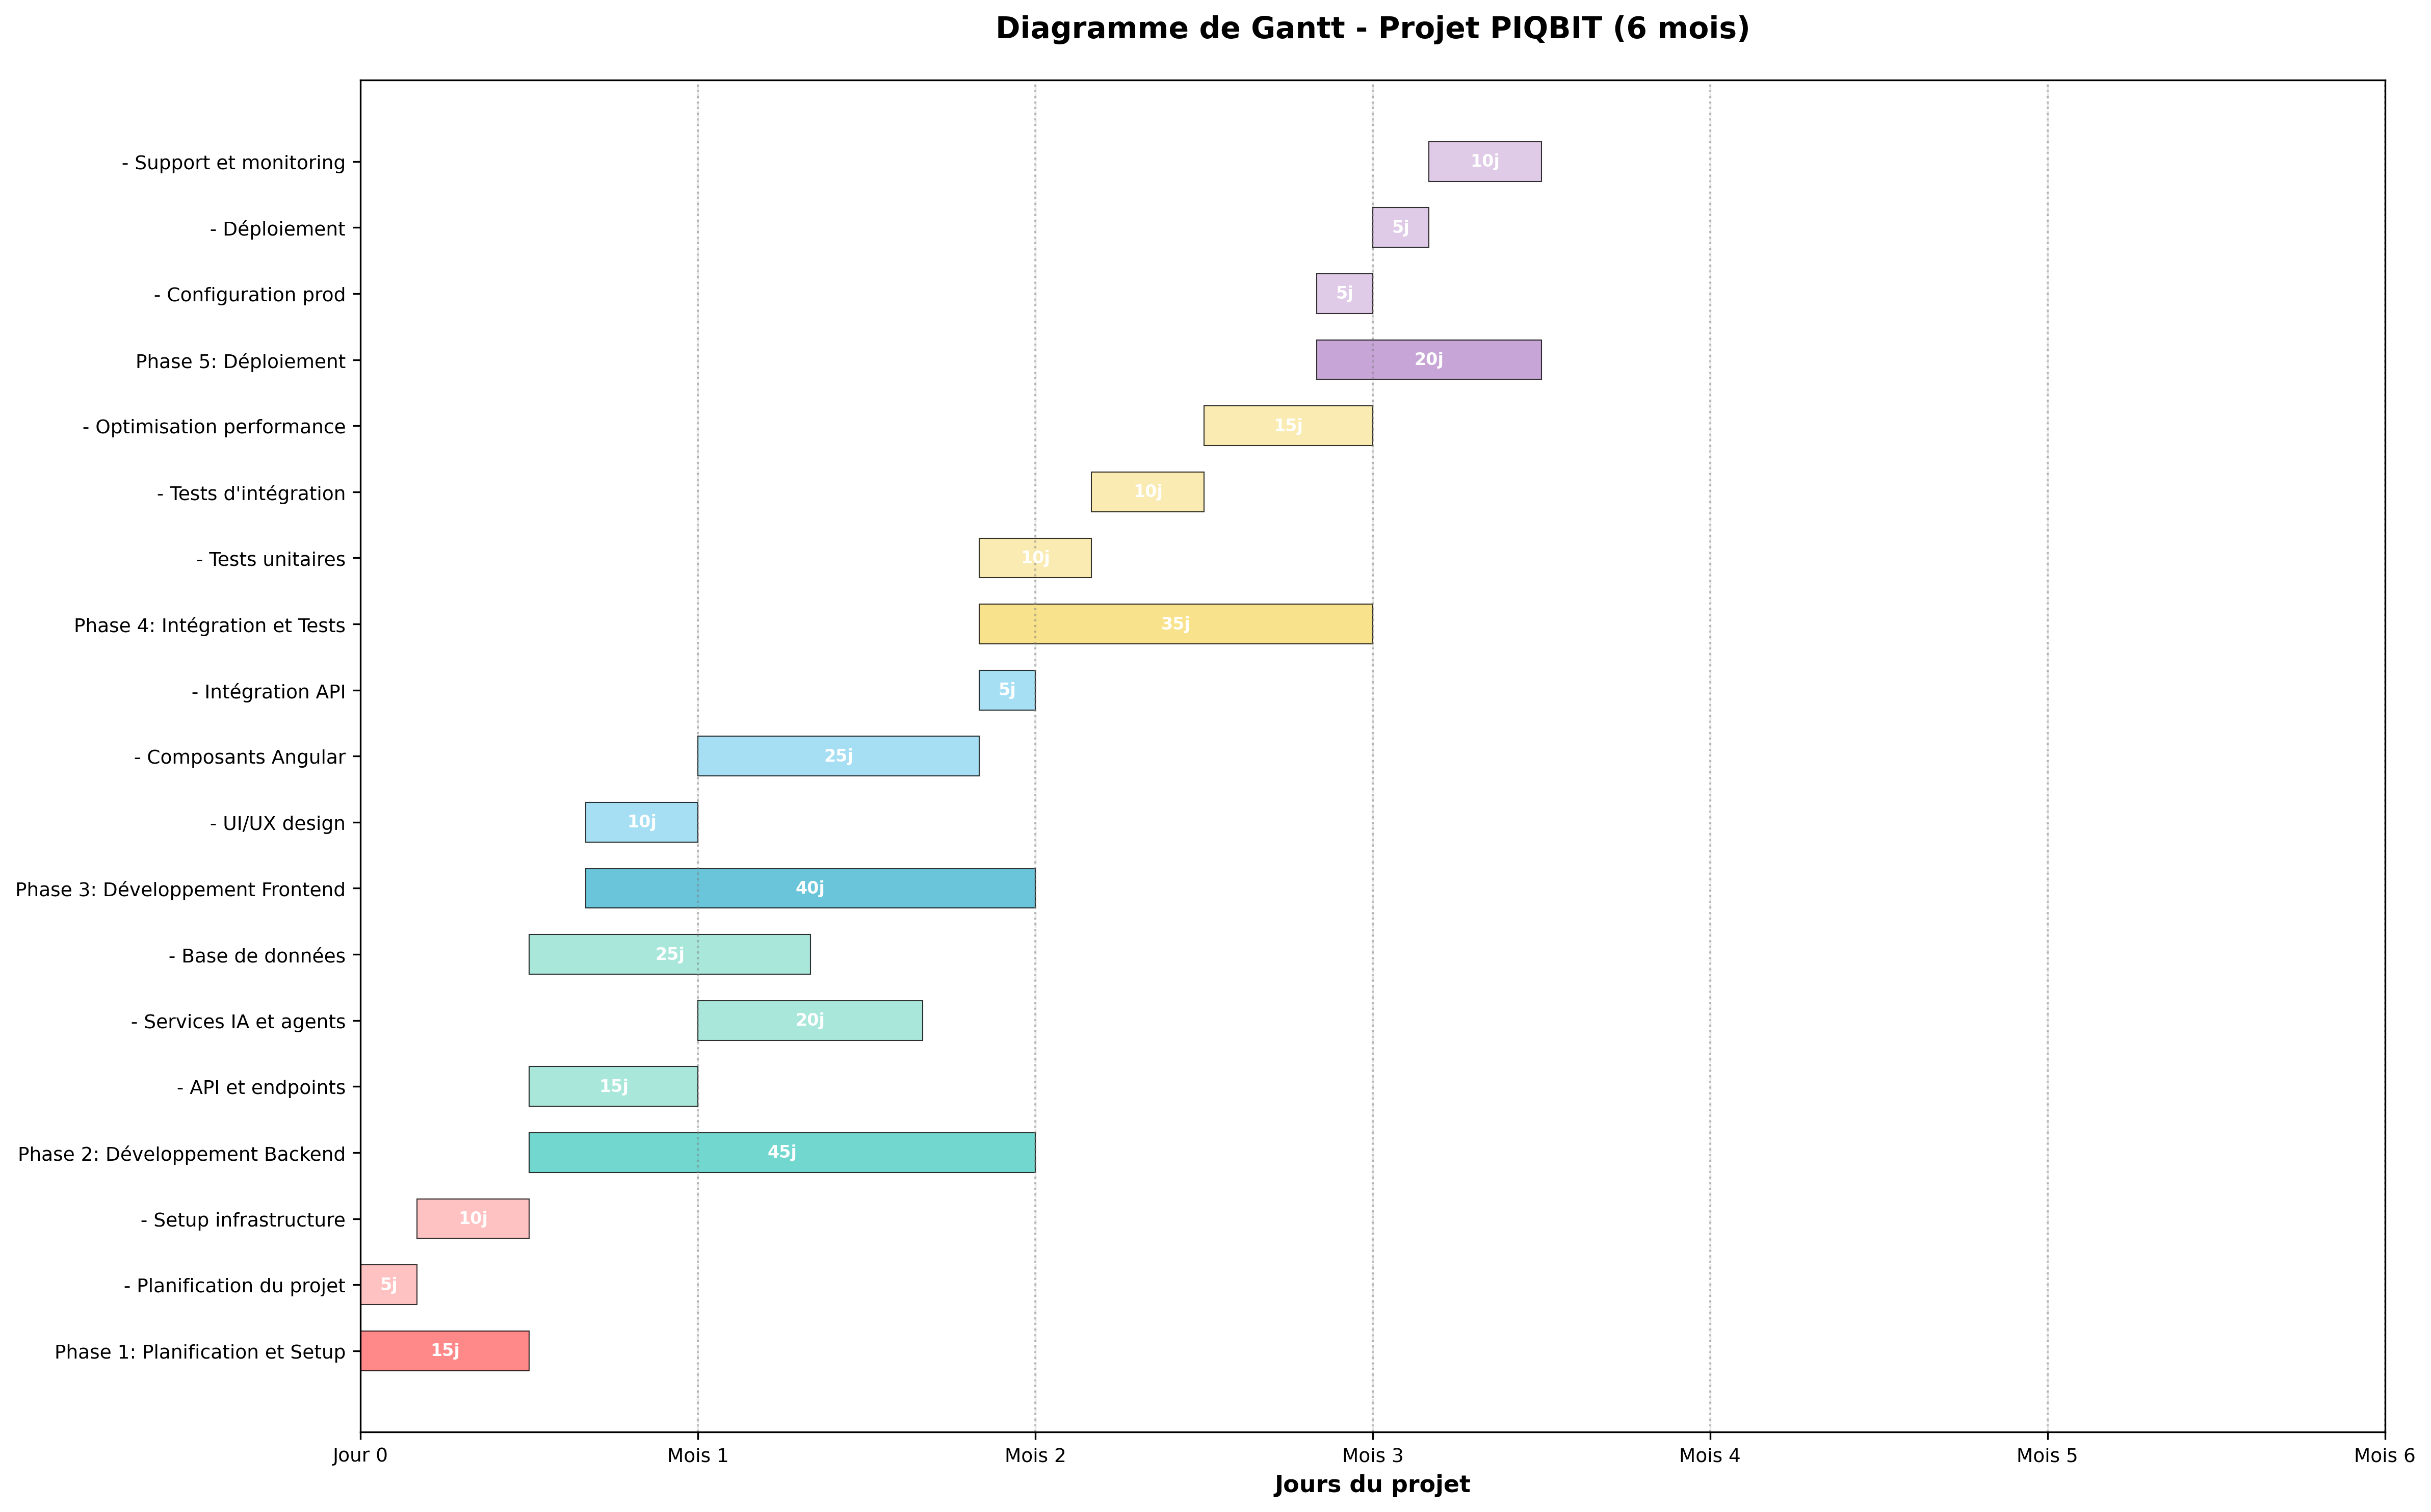
\includegraphics[width=\textwidth,keepaspectratio]{gantt_previsionnel}
  \caption[Diagramme de Gantt prévisionnel]{Diagramme de Gantt
    \textbf{prévisionnel} du projet, sur un horizon de 180 jours. Cette figure
    décrit une \emph{intention} de planification et non un déroulement
    constaté. Son découpage en cinq phases techniques ne coïncide pas avec les
    neuf phases fonctionnelles du tableau~\ref{tab:phases} : les deux
    plannings coexistent dans les sources du projet.}
  \label{fig:gantt_previsionnel}
\end{figure}

\champARemplir{Deux points à confirmer avant le dépôt. (1) Lequel des deux
découpages — neuf phases fonctionnelles ou cinq phases techniques — a
réellement guidé le travail ? Conserver celui-là et supprimer l'autre. (2) Si
vous avez tenu un suivi itératif (tableau de tâches, carnet, jalons datés),
l'ajouter ici ; sans trace, ne revendiquez pas de méthode agile — un jury
vérifie cette affirmation.}

\section{Conclusion du chapitre}
\label{sec:ctx_conclusion}

Ce chapitre a posé le contexte du recrutement assisté, montré que les
solutions existantes séparent la lecture du CV de la décision qu'elle devrait
éclairer, et formulé la problématique en termes d'automatisation
\emph{explicable}. Il a présenté le positionnement de PIQBIT, ses objectifs,
son périmètre et ses limites constatées.

Le chapitre suivant transforme ce cadrage en exigences : il identifie les
acteurs, formalise les exigences fonctionnelles et non fonctionnelles, décrit
les cas d'utilisation principaux et établit la base de traçabilité qui reliera
chaque exigence à son implémentation et à sa validation.

% ===========================================================================
% Chapitre 2 — Ingénierie des exigences.
%
% Les identifiants FR-* sont ceux du projet. Ils sont repris tels quels au
% chapitre 4 (traçabilité d'implémentation) et au chapitre 5 (validation) :
% ne les renuméroter qu'en cascade.
% ===========================================================================
\chapter{Ingénierie des exigences}
\label{chap:requirements}

\section{Introduction}
\label{sec:req_intro}

Ce chapitre transforme le cadrage du chapitre précédent en exigences
vérifiables. Il identifie les acteurs et leurs interactions, expose la méthode
de recueil, énonce les exigences fonctionnelles par domaine et les exigences
non fonctionnelles avec leurs critères d'acceptation, décrit les cas
d'utilisation principaux, et établit le modèle de traçabilité qui relie chaque
exigence à sa réalisation et à sa validation.

\section{Parties prenantes et acteurs}
\label{sec:actors}

Le tableau~\ref{tab:actors} recense les acteurs de la plateforme et leurs
interactions principales.

\begin{table}[htbp]
  \centering
  \caption{Acteurs de PIQBIT et interactions principales}
  \label{tab:actors}
  \begin{tabularx}{\textwidth}{L{2.8cm} L{4.0cm} X}
    \toprule
    \textbf{Acteur} & \textbf{Description} & \textbf{Interactions principales} \\
    \midrule
    Visiteur
      & Personne non authentifiée parcourant le site.
      & Consulter les offres publiées, rechercher, créer un compte. \\
    Candidat
      & Utilisateur authentifié déposant des candidatures.
      & Déposer un CV, postuler, suivre ses candidatures, consulter l'analyse de son CV, retirer une candidature. \\
    Porteur de lien
      & Personne agissant sans compte, au moyen d'un jeton reçu par courriel.
      & Confirmer un créneau d'entretien, passer le test technique, signer ou refuser un contrat. \\
    Recruteur
      & Rôle interne conduisant l'évaluation des candidats.
      & Consulter le classement, planifier et évaluer des entretiens, consulter les analyses de CV. \\
    Responsable RH
      & Rôle interne pilotant le recrutement et l'embauche.
      & Publier des offres, décider, éditer des contrats, piloter employés, budgets et carrières. \\
    Administrateur
      & Rôle interne d'administration du système.
      & Gérer les comptes et les rôles, consulter le journal d'audit. \\
    Traitement de fond
      & Processus asynchrones de la plateforme.
      & Analyser les CV, indexer les vecteurs, expirer les invitations, envoyer les rappels. \\
    Service externe
      & Dépendance tierce, toujours facultative.
      & Messagerie, agenda, visioconférence, modèles de langage, dépôt de modèles. \\
    \bottomrule
  \end{tabularx}
\end{table}

Le modèle de rôles implémenté comporte quatre rôles — \texttt{ADMIN},
\texttt{RH}, \texttt{RECRUTEUR}, \texttt{CANDIDAT} — liés par un héritage de
permissions : le responsable RH hérite des droits du recruteur, et
l'administrateur de ceux du responsable RH. Le « visiteur » n'est pas un rôle
stocké mais l'absence de compte ; le « porteur de lien » n'est pas davantage un
rôle : son autorisation tient au seul jeton qu'il présente, ce qui en fait une
frontière de confiance traitée à la section~\ref{sec:security_architecture}.

\section{Méthode de recueil des exigences}
\label{sec:req_method}

Les exigences proviennent de quatre sources :

\begin{enumerate}[leftmargin=*]
  \item le cahier des charges approuvé du projet, qui fixe le périmètre
        initial et les exigences non fonctionnelles chiffrées ;
  \item l'inspection du code livré — modules d'interface, services
        applicatifs, modèles de données, politique d'autorisation — qui établit
        le périmètre réellement implémenté ;
  \item les notes de conception produites pendant la réalisation, qui
        documentent les arbitrages ;
  \item les résultats de la campagne de validation, qui confirment ou
        infirment la satisfaction de chaque exigence.
\end{enumerate}

La priorisation suit un modèle MoSCoW, défini au
tableau~\ref{tab:moscow}.

\begin{table}[htbp]
  \centering
  \caption{Priorités MoSCoW retenues}
  \label{tab:moscow}
  \begin{tabularx}{\textwidth}{L{3.0cm} X}
    \toprule
    \textbf{Priorité} & \textbf{Signification dans ce projet} \\
    \midrule
    \texttt{Doit}    & Indispensable au périmètre central : sans cette capacité, la chaîne de recrutement est interrompue. \\
    \texttt{Devrait} & Important pour la complétude du produit ou pour sa validation, sans bloquer la démonstration minimale. \\
    \texttt{Pourrait}& Capacité optionnelle, réalisable après les exigences principales. \\
    \texttt{Support} & Élément implémenté qui soutient le projet sans constituer une exigence produit mise en avant. \\
    \bottomrule
  \end{tabularx}
\end{table}

\section{Exigences fonctionnelles}
\label{sec:functional_requirements}

Les exigences fonctionnelles sont groupées par domaine. Chaque groupe est
rattaché, au chapitre~\ref{chap:implementation}, à son implémentation, et au
chapitre~\ref{chap:validation}, à son résultat de validation.

\subsection{Comptes, authentification et autorisation}
\label{sec:fr_auth}

\begin{table}[htbp]
  \centering
  \caption{Exigences fonctionnelles — comptes et accès}
  \label{tab:fr_auth}
  \begin{tabularx}{\textwidth}{L{2.4cm} X L{1.9cm}}
    \toprule
    \textbf{ID} & \textbf{Exigence} & \textbf{Priorité} \\
    \midrule
    FR-AUTH-01 & Le système doit permettre l'inscription par adresse et mot de passe, la vérification de l'adresse, la connexion, la réinitialisation et le changement de mot de passe. & \texttt{Doit} \\
    FR-AUTH-02 & Le système doit proposer un second facteur d'authentification fondé sur un mot de passe à usage unique. & \texttt{Doit} \\
    FR-AUTH-03 & Le système doit plafonner les tentatives de connexion et verrouiller temporairement un compte visé. & \texttt{Doit} \\
    FR-AUTH-04 & Le système ne doit pas révéler, par sa réponse ou son temps de réponse, l'existence d'une adresse enregistrée. & \texttt{Doit} \\
    FR-AUTH-05 & Le système devrait permettre la connexion par un fournisseur d'identité externe. & \texttt{Devrait} \\
    FR-ACC-01  & Le système doit gérer quatre rôles — administrateur, responsable RH, recruteur, candidat — avec héritage de permissions. & \texttt{Doit} \\
    FR-ACC-02  & Le système doit refuser par défaut toute action non explicitement autorisée par la politique. & \texttt{Doit} \\
    FR-ACC-03  & Le système doit permettre à un utilisateur de gérer son profil, sa photo et ses coordonnées. & \texttt{Devrait} \\
    FR-ACC-04  & Le système doit journaliser les actions sensibles avec acteur, action et cible. & \texttt{Doit} \\
    FR-ACC-05  & Le système doit permettre à un utilisateur de supprimer son compte. & \texttt{Devrait} \\
    \bottomrule
  \end{tabularx}
\end{table}

Ces exigences fondent le socle. Le refus par défaut (FR-ACC-02) est structurant :
il impose que toute route nouvelle soit explicitement autorisée, plutôt que
d'être ouverte tant qu'on n'a pas pensé à la fermer.

\subsection{Offres d'emploi}
\label{sec:fr_offers}

\begin{table}[htbp]
  \centering
  \caption{Exigences fonctionnelles — offres d'emploi}
  \label{tab:fr_offers}
  \begin{tabularx}{\textwidth}{L{2.4cm} X L{1.9cm}}
    \toprule
    \textbf{ID} & \textbf{Exigence} & \textbf{Priorité} \\
    \midrule
    FR-OFF-01 & Le système doit permettre la création, la modification et la suppression d'une offre d'emploi. & \texttt{Doit} \\
    FR-OFF-02 & Une offre doit porter un intitulé, une description, des compétences requises et un statut de publication. & \texttt{Doit} \\
    FR-OFF-03 & Le système doit exposer publiquement les offres publiées, avec recherche et filtres. & \texttt{Doit} \\
    FR-OFF-04 & Le système doit permettre à un candidat d'enregistrer une offre en favori. & \texttt{Pourrait} \\
    FR-OFF-05 & Le système devrait recommander des offres à un candidat à partir de son profil. & \texttt{Devrait} \\
    \bottomrule
  \end{tabularx}
\end{table}

\subsection{Candidatures et gestion des CV}
\label{sec:fr_applications}

\begin{table}[htbp]
  \centering
  \caption{Exigences fonctionnelles — candidatures et CV}
  \label{tab:fr_applications}
  \begin{tabularx}{\textwidth}{L{2.4cm} X L{1.9cm}}
    \toprule
    \textbf{ID} & \textbf{Exigence} & \textbf{Priorité} \\
    \midrule
    FR-CAND-01 & Le système doit permettre à un candidat de postuler à une offre en joignant un CV. & \texttt{Doit} \\
    FR-CAND-02 & Le système doit contrôler le type et la taille du fichier déposé avant tout traitement. & \texttt{Doit} \\
    FR-CAND-03 & Le système doit permettre l'enregistrement d'un CV de référence réutilisable. & \texttt{Devrait} \\
    FR-CAND-04 & Le système doit exposer au candidat le statut de chacune de ses candidatures. & \texttt{Doit} \\
    FR-CAND-05 & Le système doit permettre à un candidat de retirer une candidature. & \texttt{Devrait} \\
    FR-CAND-06 & Le système doit supprimer le fichier associé lorsqu'une candidature est supprimée. & \texttt{Doit} \\
    FR-CAND-07 & Le système ne doit exposer aucune donnée personnelle de CV dans ses journaux. & \texttt{Doit} \\
    \bottomrule
  \end{tabularx}
\end{table}

L'exigence FR-CAND-07 n'est pas une précaution de confort : un CV concentre
nom, coordonnées, parcours et parfois situation familiale. Sa présence dans un
journal d'exploitation, consultable par des personnes non habilitées,
constituerait une exposition durable et difficile à corriger.

\subsection{Analyse de CV et notation}
\label{sec:fr_scoring}

\begin{table}[htbp]
  \centering
  \caption{Exigences fonctionnelles — analyse de CV et notation}
  \label{tab:fr_scoring}
  \begin{tabularx}{\textwidth}{L{2.4cm} X L{1.9cm}}
    \toprule
    \textbf{ID} & \textbf{Exigence} & \textbf{Priorité} \\
    \midrule
    FR-CV-01    & Le système doit extraire le texte d'un CV déposé en PDF ou en format bureautique. & \texttt{Doit} \\
    FR-CV-02    & Le système doit extraire du texte les compétences, l'expérience et la formation. & \texttt{Doit} \\
    FR-CV-03    & L'analyse doit s'exécuter de façon asynchrone, sans faire attendre le candidat. & \texttt{Doit} \\
    FR-SCORE-01 & Le système doit calculer un score de correspondance entre une candidature et les exigences de l'offre. & \texttt{Doit} \\
    FR-SCORE-02 & Le score doit être décomposé en sous-scores explicables et consultables. & \texttt{Doit} \\
    FR-SCORE-03 & Le système doit classer les candidats d'une offre selon leur score. & \texttt{Doit} \\
    FR-SCORE-04 & Le système doit permettre de contrôler la visibilité du score côté candidat. & \texttt{Devrait} \\
    FR-SCORE-05 & Le système devrait restituer au candidat une lecture compréhensible de l'analyse de son CV. & \texttt{Devrait} \\
    \bottomrule
  \end{tabularx}
\end{table}

FR-SCORE-02 est l'exigence centrale du projet. C'est elle qui distingue PIQBIT
d'un filtre : un score non décomposé ne serait ni justifiable devant un
candidat, ni corrigeable par un recruteur qui le juge erroné.

\subsection{Rapprochement sémantique et assistance}
\label{sec:fr_semantic}

\begin{table}[htbp]
  \centering
  \caption{Exigences fonctionnelles — sémantique et assistant}
  \label{tab:fr_semantic}
  \begin{tabularx}{\textwidth}{L{2.4cm} X L{1.9cm}}
    \toprule
    \textbf{ID} & \textbf{Exigence} & \textbf{Priorité} \\
    \midrule
    FR-SEM-01 & Le système doit indexer les CV analysés sous forme de vecteurs. & \texttt{Doit} \\
    FR-SEM-02 & Le système doit permettre la recherche de profils par proximité de sens. & \texttt{Doit} \\
    FR-SEM-03 & La recherche doit emprunter un index vectoriel natif lorsqu'il est disponible, et un repli fonctionnel sinon. & \texttt{Doit} \\
    FR-SEM-04 & Un échec d'indexation ne doit pas invalider l'analyse ni la notation. & \texttt{Doit} \\
    FR-CAG-01 & Le système doit répondre aux questions internes à partir d'une base de connaissances. & \texttt{Devrait} \\
    FR-CAG-02 & Chaque réponse doit citer les sources dont elle est extraite. & \texttt{Doit} \\
    \bottomrule
  \end{tabularx}
\end{table}

FR-CAG-02 porte une décision de conception assumée : l'assistant est
\emph{extractif} et non génératif. Il restitue des passages issus de la base et
les cite, plutôt que de formuler une réponse dont rien ne garantirait l'ancrage.

\subsection{Entretiens et évaluation}
\label{sec:fr_interviews}

\begin{table}[htbp]
  \centering
  \caption{Exigences fonctionnelles — entretiens et test technique}
  \label{tab:fr_interviews}
  \begin{tabularx}{\textwidth}{L{2.4cm} X L{1.9cm}}
    \toprule
    \textbf{ID} & \textbf{Exigence} & \textbf{Priorité} \\
    \midrule
    FR-INT-01  & Le système doit permettre de proposer jusqu'à cinq créneaux d'entretien à un candidat. & \texttt{Doit} \\
    FR-INT-02  & Le candidat doit pouvoir confirmer un créneau par un lien public, sans compte. & \texttt{Doit} \\
    FR-INT-03  & Le système doit assigner un recruteur à l'entretien et l'avertir de la confirmation. & \texttt{Doit} \\
    FR-INT-04  & Un recruteur ne doit voir que les entretiens qui lui sont affectés. & \texttt{Doit} \\
    FR-INT-05  & Le système doit générer un lien de visioconférence, avec repli si le service principal est indisponible. & \texttt{Doit} \\
    FR-INT-06  & Le système devrait synchroniser l'entretien confirmé avec un agenda externe. & \texttt{Devrait} \\
    FR-INT-07  & Le système doit expirer automatiquement les invitations restées sans réponse. & \texttt{Doit} \\
    FR-INT-08  & Le système doit permettre l'évaluation d'un entretien une fois celui-ci passé. & \texttt{Devrait} \\
    FR-TEST-01 & Le système doit proposer un test technique chronométré par lien public. & \texttt{Doit} \\
    FR-TEST-02 & Le système doit corriger automatiquement le test et en calculer le score. & \texttt{Doit} \\
    FR-TEST-03 & Le seuil d'éligibilité doit être évalué côté serveur. & \texttt{Doit} \\
    FR-TEST-04 & Le système doit clore automatiquement les sessions dont le temps est écoulé. & \texttt{Doit} \\
    \bottomrule
  \end{tabularx}
\end{table}

\subsection{Salaire, négociation et contrats}
\label{sec:fr_contracts}

\begin{table}[htbp]
  \centering
  \caption{Exigences fonctionnelles — salaire, négociation et contrats}
  \label{tab:fr_contracts}
  \begin{tabularx}{\textwidth}{L{2.4cm} X L{1.9cm}}
    \toprule
    \textbf{ID} & \textbf{Exigence} & \textbf{Priorité} \\
    \midrule
    FR-SAL-01  & Le système doit prédire une fourchette salariale à partir d'un modèle entraîné. & \texttt{Doit} \\
    FR-SAL-02  & La prédiction doit s'accompagner d'un intervalle et non d'une valeur unique. & \texttt{Devrait} \\
    FR-NEGO-01 & Le système doit enregistrer les tours successifs d'une négociation avec montants et arguments. & \texttt{Devrait} \\
    FR-NEGO-02 & Le système devrait assister le recruteur dans la formulation d'une contre-proposition. & \texttt{Devrait} \\
    FR-CTR-01  & Le système doit permettre d'éditer un contrat à partir d'une candidature retenue. & \texttt{Doit} \\
    FR-CTR-02  & Le contrat doit être signé par lien public à jeton, sans compte. & \texttt{Doit} \\
    FR-CTR-03  & Le système doit calculer une empreinte des termes signés. & \texttt{Doit} \\
    FR-CTR-04  & Le système doit produire un certificat et une piste d'audit de la signature. & \texttt{Doit} \\
    FR-CTR-05  & Un lien de signature rejoué ne doit jamais signer deux fois. & \texttt{Doit} \\
    FR-CTR-06  & La signature doit créer ou rattacher la fiche employé, sans doublon. & \texttt{Doit} \\
    \bottomrule
  \end{tabularx}
\end{table}

\subsection{Ressources humaines internes et restitution}
\label{sec:fr_hr}

\begin{table}[htbp]
  \centering
  \caption{Exigences fonctionnelles — RH interne, rapports et notifications}
  \label{tab:fr_hr}
  \begin{tabularx}{\textwidth}{L{2.4cm} X L{1.9cm}}
    \toprule
    \textbf{ID} & \textbf{Exigence} & \textbf{Priorité} \\
    \midrule
    FR-RH-01    & Le système doit gérer un répertoire des employés. & \texttt{Devrait} \\
    FR-RH-02    & Le système doit gérer des budgets par département et l'imputation des dépenses. & \texttt{Devrait} \\
    FR-RH-03    & Le système devrait gérer des plans de carrière avec objectifs et jalons. & \texttt{Pourrait} \\
    FR-REP-01   & Le système doit produire des synthèses de l'activité de recrutement. & \texttt{Devrait} \\
    FR-REP-02   & Le système devrait archiver des instantanés de ces synthèses. & \texttt{Pourrait} \\
    FR-REP-03   & Le système devrait proposer une aide à la décision comparant les candidats. & \texttt{Devrait} \\
    FR-NOTIF-01 & Le système doit notifier les acteurs des événements les concernant. & \texttt{Doit} \\
    FR-NOTIF-02 & Les notifications doivent être diffusées en temps réel sur une liaison authentifiée. & \texttt{Devrait} \\
    \bottomrule
  \end{tabularx}
\end{table}

\section{Exigences non fonctionnelles}
\label{sec:nonfunctional_requirements}

Le tableau~\ref{tab:nfr} énonce les exigences non fonctionnelles avec leur
critère d'acceptation et leur état de vérification au
22~septembre~2026. Cet état est repris et démontré au
chapitre~\ref{chap:validation}.

\begin{table}[htbp]
  \centering
  \caption{Exigences non fonctionnelles et état de vérification}
  \label{tab:nfr}
  \begin{tabularx}{\textwidth}{L{1.9cm} L{2.5cm} X L{2.2cm}}
    \toprule
    \textbf{ID} & \textbf{Catégorie} & \textbf{Critère d'acceptation} & \textbf{État} \\
    \midrule
    NFR-01 & Sécurité      & Les mots de passe sont hachés par une fonction lente et salée. & Vérifiée \\
    NFR-02 & Sécurité      & Toute action sensible est refusée par défaut sans autorisation explicite. & \textbf{Écart constaté} \\
    NFR-03 & Sécurité      & Les jetons publics font au moins 32 octets d'entropie. & Vérifiée \\
    NFR-04 & Confidentialité & Aucune donnée personnelle de CV n'apparaît dans les journaux. & Vérifiée \\
    NFR-05 & Fiabilité     & L'indisponibilité d'un service externe ne bloque aucun parcours. & Vérifiée \\
    NFR-06 & Intégrité     & Le schéma de la base est piloté exclusivement par migrations. & Vérifiée \\
    NFR-07 & Performance   & Le dépôt d'une candidature répond sans attendre l'analyse du CV. & Vérifiée \\
    NFR-08 & Performance   & Le bundle initial du client reste sous le budget fixé. & \textbf{Non satisfaite} \\
    NFR-09 & Maintenabilité & Le code est typé et validé aux frontières. & Vérifiée \\
    NFR-10 & Disponibilité & Le service atteint 99,5\,\% de disponibilité en production. & \textbf{Non vérifiée} \\
    NFR-11 & Accessibilité & L'interface respecte les critères d'accessibilité retenus. & \textbf{Non vérifiée} \\
    \bottomrule
  \end{tabularx}
\end{table}

Trois exigences ne sont pas satisfaites, et le rapport les traite comme telles.
NFR-08 est mesurée en dépassement. NFR-10 et NFR-11 ne sont pas vérifiées faute
d'environnement de production et de campagne d'accessibilité : les déclarer
vérifiées serait une affirmation sans preuve. NFR-02 présente un écart révélé
par la campagne de validation, analysé à la
section~\ref{sec:failure_analysis}.

\section{Cas d'utilisation}
\label{sec:use_cases}

La figure~\ref{fig:use_cases} donne la vue d'ensemble des cas d'utilisation et
de leurs acteurs.

\pqfigure{use_cases}
  {Diagramme de cas d'utilisation de PIQBIT : acteurs, capacités et héritage
   de permissions entre rôles internes.}
  {fig:use_cases}

\subsection{Décomposition détaillée des cas principaux}
\label{sec:use_cases_detail}

Le tableau~\ref{tab:use_case_catalog} catalogue les cas d'utilisation
principaux, puis quatre d'entre eux sont détaillés.

\begin{table}[htbp]
  \centering
  \caption{Catalogue des cas d'utilisation principaux}
  \label{tab:use_case_catalog}
  \begin{tabularx}{\textwidth}{L{1.7cm} L{4.6cm} L{3.0cm} X}
    \toprule
    \textbf{ID} & \textbf{Cas d'utilisation} & \textbf{Acteur principal} & \textbf{Exigences} \\
    \midrule
    UC-01 & Postuler à une offre                  & Candidat        & FR-CAND-01/02 \\
    UC-02 & Analyser et noter une candidature     & Traitement de fond & FR-CV-01/02/03, FR-SCORE-01/02/03 \\
    UC-03 & Consulter le classement des candidats & Recruteur       & FR-SCORE-03 \\
    UC-04 & Rechercher un profil par le sens      & Recruteur       & FR-SEM-01/02/03 \\
    UC-05 & Planifier un entretien                & Recruteur       & FR-INT-01/03 \\
    UC-06 & Confirmer un créneau d'entretien      & Porteur de lien & FR-INT-02/05 \\
    UC-07 & Passer le test technique              & Porteur de lien & FR-TEST-01/02 \\
    UC-08 & Estimer un salaire et négocier        & Responsable RH  & FR-SAL-01, FR-NEGO-01 \\
    UC-09 & Signer un contrat                     & Porteur de lien & FR-CTR-02/03/04/05 \\
    UC-10 & Activer la fiche employé              & Système         & FR-CTR-06 \\
    UC-11 & Administrer comptes et rôles          & Administrateur  & FR-ACC-01/02/04 \\
    \bottomrule
  \end{tabularx}
\end{table}

\paragraph{UC-01 — Postuler à une offre.}
\emph{Acteur :} candidat authentifié. \emph{Précondition :} l'offre est
publiée et le candidat n'y a pas déjà postulé. \emph{Scénario nominal :} le
candidat ouvre la fiche de l'offre, joint un CV ou réutilise son CV de
référence, valide ; le système contrôle le type et la taille du fichier,
enregistre la candidature, planifie l'analyse et répond immédiatement.
\emph{Variantes :} format non accepté ou taille excessive — la candidature est
refusée avec un message explicite. \emph{Postcondition :} la candidature existe
au statut initial et son analyse est planifiée.

\paragraph{UC-02 — Analyser et noter une candidature.}
\emph{Acteur :} traitement de fond. \emph{Précondition :} une candidature vient
d'être déposée. \emph{Scénario nominal :} le traitement extrait le texte du CV,
en tire compétences, expérience et formation, enregistre l'analyse, indexe les
vecteurs, calcule le score et reclasse les candidats de l'offre.
\emph{Variantes :} l'indexation échoue — la notation est conservée, la
recherche sémantique sera simplement moins riche. \emph{Postcondition :} la
candidature porte une analyse, un score décomposé et un rang.

\paragraph{UC-06 — Confirmer un créneau d'entretien.}
\emph{Acteur :} porteur de lien, sans compte. \emph{Précondition :} une
invitation est active et non expirée. \emph{Scénario nominal :} le porteur
ouvre le lien reçu, consulte les créneaux, en choisit un ; le système vérifie
que le créneau n'a pas été réservé entre-temps, marque l'invitation confirmée,
avertit le recruteur assigné et synchronise l'agenda.
\emph{Variantes :} lien expiré, déjà confirmé ou annulé — l'action est refusée
avec une raison distincte dans chaque cas. \emph{Postcondition :} l'entretien
est confirmé et le recruteur assigné en est informé.

\paragraph{UC-09 — Signer un contrat.}
\emph{Acteur :} porteur de lien, sans compte. \emph{Précondition :} un contrat
a été envoyé et n'est ni signé, ni refusé. \emph{Scénario nominal :} le porteur
ouvre le lien, consulte les termes en lecture seule, saisit son nom et son
tracé de signature ; le système vérifie l'état du contrat, calcule l'empreinte
des termes, émet un certificat, enregistre la piste d'audit, puis crée ou
rattache la fiche employé. \emph{Variantes :} contrat déjà signé — refus
explicite ; lien rejoué — aucune seconde signature. \emph{Postcondition :} le
contrat est signé, certifié, et la fiche employé est active.

\section{Acceptation et traçabilité}
\label{sec:traceability}

Chaque exigence est reliée à son implémentation et à sa validation selon le
modèle du tableau~\ref{tab:traceability_model}. La matrice complète figure en
annexe~\ref{app:traceability}.

\begin{table}[htbp]
  \centering
  \caption{Modèle de traçabilité des exigences}
  \label{tab:traceability_model}
  \begin{tabularx}{\textwidth}{L{3.4cm} X}
    \toprule
    \textbf{Élément} & \textbf{Contenu} \\
    \midrule
    Identifiant d'exigence & Référence stable, réutilisée sans modification aux chapitres 4 et 5 \\
    Domaine                & Groupe fonctionnel d'appartenance \\
    Implémentation         & Sous-système du chapitre~\ref{chap:implementation} qui réalise l'exigence \\
    Validation             & Résultat daté du chapitre~\ref{chap:validation} \\
    État                   & Satisfaite, partiellement satisfaite, non satisfaite ou non vérifiée \\
    \bottomrule
  \end{tabularx}
\end{table}

Le vocabulaire d'état est volontairement restreint. « Non vérifiée » n'est pas
un synonyme atténué de « satisfaite » : il signale qu'aucune preuve n'existe,
ce qui est une information en soi.

\section{Limites de périmètre}
\label{sec:scope_boundaries}

Les éléments suivants sont explicitement hors périmètre :

\begin{itemize}[leftmargin=*]
  \item l'analyse de CV en langues autres que celles couvertes par le modèle
        de plongement retenu ;
  \item la détection de fraude documentaire sur les CV ;
  \item l'intégration avec des jobboards externes pour la diffusion des offres ;
  \item la paie et la gestion administrative des employés au-delà de la fiche
        et du budget ;
  \item la conformité juridique de la signature électronique au sens d'un
        règlement de signature qualifiée : la signature implémentée est
        auto-hébergée, avec empreinte et piste d'audit, ce qui en fait une
        preuve d'intention et non une signature qualifiée.
\end{itemize}

\section{Conclusion du chapitre}
\label{sec:req_conclusion}

Ce chapitre a identifié les acteurs de PIQBIT, formalisé les exigences
fonctionnelles en huit domaines et les exigences non fonctionnelles avec leurs
critères d'acceptation, décrit les cas d'utilisation principaux et posé le
modèle de traçabilité. Trois exigences non fonctionnelles sont d'ores et déjà
identifiées comme non satisfaites ou non vérifiées, ce que le
chapitre~\ref{chap:validation} documentera par des mesures datées.

Le chapitre suivant traduit ces exigences en architecture : contexte système,
découpage en composants, modèle de données, séquences principales, frontières
de sécurité et décisions d'architecture justifiées.

% ===========================================================================
% Chapitre 3 — Architecture et conception.
% Toute la matière de ce chapitre est relevée dans le dépôt au 2026-09-22.
% ===========================================================================
\chapter{Architecture et conception}
\label{chap:architecture}

\section{Introduction}
\label{sec:arch_intro}

Ce chapitre traduit les exigences du chapitre précédent en une architecture.
Il énonce d'abord les objectifs architecturaux et les réponses apportées,
délimite le système et ses dépendances, décrit le découpage en composants et
le modèle de données, expose les séquences des deux parcours les plus
structurants, analyse les frontières de confiance, décrit le déploiement, et
consigne enfin les décisions d'architecture avec leurs alternatives écartées.

\section{Objectifs architecturaux}
\label{sec:arch_objectives}

Le tableau~\ref{tab:arch_objectives} associe à chaque objectif architectural
la réponse retenue.

\begin{table}[htbp]
  \centering
  \caption{Objectifs architecturaux et réponses apportées}
  \label{tab:arch_objectives}
  \begin{tabularx}{\textwidth}{L{3.6cm} X}
    \toprule
    \textbf{Objectif} & \textbf{Réponse architecturale} \\
    \midrule
    Explicabilité      & Le score est stocké décomposé en sous-scores persistés, non recalculé à l'affichage : ce qui a été montré au recruteur reste consultable ensuite. \\
    Réactivité perçue  & Les traitements longs — analyse de CV, indexation — s'exécutent hors du cycle de la requête, dans une session de base dédiée. \\
    Résilience         & Toute dépendance externe est facultative et dotée d'un repli implémenté ; aucune n'est sur le chemin critique. \\
    Sécurité           & Politique d'autorisation externalisée, refus par défaut, et traitement des liens publics à jeton comme une frontière de confiance à part entière. \\
    Intégrité du schéma& Le schéma est piloté exclusivement par migrations ; l'application vérifie la révision au démarrage et refuse de servir un schéma désynchronisé. \\
    Confidentialité    & Aucune donnée personnelle de CV n'est écrite dans les journaux, à aucun niveau de verbosité. \\
    \bottomrule
  \end{tabularx}
\end{table}

\section{Contexte système}
\label{sec:system_context}

La figure~\ref{fig:system_context} délimite le système, ses acteurs et ses
dépendances externes. Le tableau~\ref{tab:external_deps} détaille chaque
dépendance et son repli.

\pqfigure{system_context}
  {Frontière du système PIQBIT, acteurs et dépendances externes. Le trait
   discontinu marque une dépendance \emph{facultative} dotée d'un repli
   implémenté.}
  {fig:system_context}

\begin{table}[htbp]
  \centering
  \caption{Dépendances externes et comportement de repli}
  \label{tab:external_deps}
  \begin{tabularx}{\textwidth}{L{3.2cm} L{4.2cm} X}
    \toprule
    \textbf{Dépendance} & \textbf{Usage} & \textbf{Comportement si indisponible} \\
    \midrule
    Serveur SMTP     & Invitations, confirmations, rappels & Le message est journalisé au lieu d'être émis ; le parcours se poursuit \\
    Google Calendar  & Synchronisation des entretiens confirmés & Un fichier \texttt{.ics} téléchargeable remplace la synchronisation \\
    Google Meet      & Lien de visioconférence & \textbf{Aucun repli} : sans compte Google rattaché au recruteur désigné, aucun lien n'est créé et aucun rappel de connexion n'est envoyé \\
    Google OAuth     & Connexion par identité externe & La connexion par mot de passe reste disponible \\
    Modèles de langage & Enrichissement de l'assistant & L'assistant reste extractif : il cite la base, sans reformulation \\
    Dépôt de modèles & Téléchargement du modèle de plongement & Le cache local est employé ; à défaut, la recherche sémantique est désactivée sans bloquer la notation \\
    \bottomrule
  \end{tabularx}
\end{table}

Cette propriété a un coût qu'il faut énoncer : des chemins de repli moins
éprouvés que le chemin nominal. La campagne de validation n'a ainsi exercé que
le repli de la recherche sémantique, et non son chemin vectoriel natif
(section~\ref{sec:validation_results}).

\section{Architecture en composants}
\label{sec:component_view}

La figure~\ref{fig:component_view} présente le découpage en composants, et le
tableau~\ref{tab:components} les responsabilités de chaque couche.

\pqfigure{component_view}
  {Vue logique en composants : client Angular, frontière HTTP, couche API,
   services applicatifs et persistance. Relevé du 22 septembre 2026.}
  {fig:component_view}

\begin{table}[htbp]
  \centering
  \caption{Composants de PIQBIT et responsabilités}
  \label{tab:components}
  \begin{tabularx}{\textwidth}{L{3.4cm} X}
    \toprule
    \textbf{Composant} & \textbf{Responsabilité} \\
    \midrule
    Client Angular       & Interfaces front-office, back-office et pages publiques ; chargement différé des modules lourds \\
    Serveur statique     & Service du bundle, relais des appels d'interface et des liaisons temps réel, en-têtes de sécurité \\
    Couche API           & 18 modules d'endpoints exposant 173 routes et deux points de liaison temps réel \\
    Authentification     & Vérification du jeton, second facteur, identité externe \\
    Autorisation         & Décision d'accès par rôle, refus par défaut \\
    Validation           & Contrôle des entrées aux frontières par schémas typés \\
    Services applicatifs & 33 modules portant les règles métier de chaque domaine \\
    Intégrations         & Trois clients vers les services externes, tous facultatifs \\
    Accès aux données    & Correspondance objet-relationnel asynchrone sur 25 tables \\
    \bottomrule
  \end{tabularx}
\end{table}

La règle de dépendance est unidirectionnelle : l'interface appelle l'API, qui
appelle les services, qui appellent la persistance. Un service n'appelle jamais
un endpoint, et la persistance ne connaît aucune couche supérieure. Cette
discipline rend chaque couche testable indépendamment.

\section{Couche applicative et interfaces}
\label{sec:interfaces}

Le tableau~\ref{tab:backend_modules} récapitule les modules d'endpoints et
leur rôle architectural.

\begin{table}[htbp]
  \centering
  \caption{Modules d'endpoints et rôles architecturaux}
  \label{tab:backend_modules}
  \begin{tabularx}{\textwidth}{L{3.4cm} X}
    \toprule
    \textbf{Module} & \textbf{Rôle} \\
    \midrule
    Authentification  & Inscription, connexion, second facteur, réinitialisation, identité externe \\
    Comptes           & Profils, rôles, photo, journal d'audit, suppression de compte \\
    Recrutement       & Offres, candidatures, dépôt et gestion des CV \\
    Notation          & Analyse de CV, scores, classement \\
    Sémantique        & Indexation vectorielle et recherche par proximité de sens \\
    Assistant         & Interrogation de la base de connaissances, réponses sourcées \\
    Entretiens        & Invitations, créneaux, confirmation publique, agenda, visioconférence \\
    Évaluation        & Questions, sessions de test, correction, résultats \\
    Négociation       & Tours d'échange, assistance à la contre-proposition \\
    Contrats          & Édition, envoi, signature publique, certificat \\
    Employés          & Répertoire et fiches employé \\
    Budget            & Enveloppes par département et imputation des dépenses \\
    Carrière          & Objectifs et jalons de progression \\
    Rapports          & Synthèses et instantanés archivés \\
    Décision          & Comparaison de candidats et aide au choix \\
    Notifications     & Diffusion en temps réel et historique \\
    Tableau de bord   & Indicateurs agrégés du back-office \\
    Flux de travail   & Transitions de statut des candidatures \\
    \bottomrule
  \end{tabularx}
\end{table}

Les conventions d'interface sont uniformes : validation des entrées par schémas
typés~\cite{pydantic}, codes de statut normalisés, et identifiants universels comme clés
externes. Deux points de liaison temps réel complètent les routes : l'un pour
les notifications, l'autre pour la négociation, tous deux authentifiés par
jeton — une liaison persistante ne portant pas les en-têtes d'une requête
ordinaire.

\section{Modèle de données et persistance}
\label{sec:data_model}

Le modèle comporte 25 tables, groupées par domaine
(figure~\ref{fig:domain_model}). Le tableau~\ref{tab:domain_groups} en résume
les responsabilités.

\pqfigurewide{domain_model}
  {Modèle de données : 25 tables groupées par domaine. Les cardinalités
   proviennent des contraintes réelles ; deux liens non contraints par le
   moteur sont signalés.}
  {fig:domain_model}

\begin{table}[htbp]
  \centering
  \caption{Groupes du domaine et responsabilités de persistance}
  \label{tab:domain_groups}
  \begin{tabularx}{\textwidth}{L{3.4cm} L{2.0cm} X}
    \toprule
    \textbf{Groupe} & \textbf{Tables} & \textbf{Responsabilité} \\
    \midrule
    Identité et accès    & 2 & Comptes, rôles, second facteur, journal d'audit \\
    Recrutement          & 4 & Candidats, offres, candidatures, favoris \\
    Analyse et notation  & 4 & Analyses de CV, scores, vecteurs et segments indexés \\
    Évaluation           & 5 & Invitations, créneaux, questions, sessions et réponses de test \\
    Embauche             & 4 & Négociations, tours, contrats, employés \\
    RH interne et diffusion & 4 & Budgets, dépenses, plans de carrière, notifications \\
    Instantanés          & 2 & Rapports archivés et bases de connaissances \\
    \bottomrule
  \end{tabularx}
\end{table}

\paragraph{Décision D-01 — le schéma est piloté par migrations.}
Les révisions sont gérées par Alembic~\cite{alembic}, l'outil de migration
associé à la couche de persistance~\cite{sqlalchemy}.
Le schéma n'est jamais créé ni modifié par l'application. Au démarrage,
celle-ci \emph{vérifie} que la base porte la dernière révision de migration et
journalise une erreur explicite en cas d'écart. L'alternative écartée — la
création automatique des tables au démarrage — produit une dérive silencieuse
entre environnements : une colonne ajoutée en développement apparaît sans
migration, et son absence en production ne se découvre qu'au premier appel qui
la touche. Le critère retenu est l'absence de dérive, garantie par un contrôle
en intégration continue qui compare les migrations aux modèles.

\section{Séquences principales}
\label{sec:dynamic_views}

Deux parcours portent l'essentiel de la dynamique du système.

\subsection{Candidature, analyse et notation}

La figure~\ref{fig:sequence_scoring} détaille le parcours du dépôt d'une
candidature jusqu'au classement du candidat.

\pqfigure{sequence_scoring}
  {Candidature, analyse de CV, notation et classement. La réponse
   \texttt{201} part avant le traitement : l'analyse s'exécute en tâche de
   fond, dans une session de base dédiée.}
  {fig:sequence_scoring}

Le point de conception à retenir est la frontière asynchrone. La réponse est
émise dès la candidature enregistrée, avant l'analyse — qui prend plusieurs
secondes. Cela impose deux contraintes : la tâche de fond doit ouvrir sa propre
session de base, celle de la requête étant déjà fermée ; et l'interface doit
représenter un état transitoire, l'analyse n'étant pas immédiatement
disponible. Le bénéfice est une latence perçue constante, indépendante de la
taille du CV.

\subsection{Contrat, signature et activation de l'employé}

La figure~\ref{fig:sequence_contract} détaille la signature d'un contrat par
lien public.

\pqfigure{sequence_contract_signature}
  {Contrat, signature par lien à jeton et activation de l'employé. Le jeton
   tient lieu d'authentification : les gardes d'état précèdent toute écriture.}
  {fig:sequence_contract}

Deux propriétés sont conçues explicitement. D'une part les \emph{gardes
d'état} : un contrat déjà signé, refusé, ou dans un état autre qu'envoyé, est
rejeté avec un code distinct selon le cas — un lien rejoué ne signe jamais deux
fois. D'autre part l'\emph{idempotence} de la création d'employé : la fiche est
recherchée par adresse avant d'être créée, ce qui évite les doublons si
l'opération est rejouée.

\section{Sécurité et frontières de confiance}
\label{sec:security_architecture}

La figure~\ref{fig:security_view} distingue les deux chemins d'entrée du
système, et le tableau~\ref{tab:security_controls} récapitule les contrôles.
Les frontières retenues suivent les catégories de risque du référentiel
OWASP~\cite{owasptop10}, en particulier le contrôle d'accès défaillant et
l'exposition de données sensibles.

\pqfigure{security_view}
  {Frontières de confiance. Deux chemins d'entrée coexistent : authentifié
   (jeton signé, second facteur, autorisation) et public à jeton — neuf routes
   où le jeton tient lieu d'authentification.}
  {fig:security_view}

\begin{table}[htbp]
  \centering
  \caption{Frontières de confiance et contrôles associés}
  \label{tab:security_controls}
  \begin{tabularx}{\textwidth}{L{3.4cm} X}
    \toprule
    \textbf{Frontière} & \textbf{Contrôle} \\
    \midrule
    Entrée réseau        & En-têtes de sécurité, origine unique. \textbf{Aucune terminaison TLS} dans la composition fournie \\
    Authentification     & Jeton signé à durée limitée ; second facteur par mot de passe à usage unique \\
    Autorisation         & Politique déclarative externalisée, refus par défaut, héritage de rôles \\
    Liens publics à jeton& Jeton de 32 octets imprévisible, gardes d'état avant écriture, durée de validité bornée \\
    Dépôt de fichiers    & Liste blanche de types et plafond de taille appliqués avant tout traitement \\
    Journalisation       & Aucune donnée personnelle de CV, à aucun niveau de verbosité \\
    Piste d'audit        & Acteur, action et cible consignés pour les opérations sensibles \\
    \bottomrule
  \end{tabularx}
\end{table}

\paragraph{Décision D-02 — la politique d'autorisation est externalisée.}
Les droits sont décrits dans un fichier déclaratif, et non dispersés en
conditions dans le code. La politique parle du métier — « le recruteur peut
lire les candidatures » — plutôt que des routes ; chaque endpoint déclare la
ressource et l'action qu'il engage. L'alternative écartée — un contrôle écrit
sur les chemins et les verbes — se désynchronise au premier renommage de route
et se relit mal. Le critère retenu est l'auditabilité : la politique complète
se lit dans un seul fichier, ce que la section~\ref{sec:failure_analysis}
montre justement utile lorsqu'un écart survient.

\paragraph{Les liens publics à jeton sont une frontière à part entière.}
Neuf routes acceptent un jeton en guise d'authentification : confirmation
d'entretien, passage de test, signature et refus de contrat. C'est un choix
fonctionnel — exiger un compte d'un candidat pour confirmer un créneau
ajouterait une friction disproportionnée — mais il déplace la sécurité du
porteur vers le jeton. D'où trois exigences de conception : entropie suffisante
(32 octets), validité bornée dans le temps, et gardes d'état systématiques
avant toute écriture.

\section{Vue de déploiement}
\label{sec:deployment_view}

La figure~\ref{fig:deployment_view} restitue la composition de
conteneurs~\cite{docker} au 22 septembre 2026.

\pqfigure{deployment_view}
  {Vue de déploiement. Le conteneur applicatif ne publie aucun port : il n'est
   atteignable qu'à travers le serveur statique. Aucune terminaison TLS, aucun
   environnement cible.}
  {fig:deployment_view}

Trois constats doivent être énoncés sans détour. Le conteneur applicatif
\emph{ne publie aucun port} vers l'hôte : il n'est joignable qu'à travers le
serveur statique, et c'est une propriété voulue. En revanche, la composition
\emph{ne comporte aucune terminaison TLS} : le point d'entrée est en clair. Et
\emph{aucun environnement d'hébergement cible} n'existe à ce jour : la
composition décrite est celle du poste de développement, sans procédure de
retour arrière définie.

\section{Décisions d'architecture}
\label{sec:architecture_decisions}

Le tableau~\ref{tab:arch_decisions} récapitule les décisions structurantes.
Chacune énonce l'alternative écartée et le critère d'arbitrage, faute de quoi
une décision n'est qu'une préférence.

\begin{table}[htbp]
  \centering
  \caption{Décisions d'architecture principales}
  \label{tab:arch_decisions}
  \begin{tabularx}{\textwidth}{L{1.3cm} L{3.4cm} X}
    \toprule
    \textbf{Réf.} & \textbf{Décision} & \textbf{Alternative écartée et critère} \\
    \midrule
    D-01 & Schéma piloté par migrations, vérifié au démarrage
         & \emph{Écarté :} création automatique des tables. \emph{Critère :} absence de dérive entre environnements \\
    D-02 & Politique d'autorisation externalisée, refus par défaut
         & \emph{Écarté :} contrôles dispersés par route. \emph{Critère :} auditabilité en un seul fichier \\
    D-03 & Recherche vectorielle native, avec repli applicatif
         & \emph{Écarté :} dépendance stricte à l'extension vectorielle. \emph{Critère :} la plateforme doit rester utilisable sans elle \\
    D-04 & Sélection du modèle salarial sur l'erreur de \emph{test}
         & \emph{Écarté :} sélection sur l'erreur d'entraînement. \emph{Critère :} un modèle qui mémorise se repère uniquement en test \\
    D-05 & Retrait d'une variable colinéaire du modèle
         & \emph{Écarté :} conservation de toutes les variables. \emph{Critère :} la colinéarité créait un mode de défaillance identifié \\
    D-06 & Assistant \emph{extractif} citant ses sources
         & \emph{Écarté :} génération libre. \emph{Critère :} une réponse non ancrée n'est pas vérifiable par le lecteur \\
    D-07 & Signature auto-hébergée avec empreinte et certificat
         & \emph{Écarté :} prestataire de signature externe. \emph{Critère :} maîtrise de la piste d'audit ; limite juridique assumée \\
    D-08 & Analyse de CV asynchrone, en session dédiée
         & \emph{Écarté :} analyse synchrone. \emph{Critère :} latence perçue indépendante de la taille du document \\
    \bottomrule
  \end{tabularx}
\end{table}

\section{Conclusion du chapitre}
\label{sec:arch_conclusion}

Ce chapitre a établi l'architecture de PIQBIT : un découpage en couches à
dépendance unidirectionnelle, un modèle de 25 tables piloté par migrations,
deux chemins d'entrée dont un public à jeton traité comme frontière de
confiance, et huit décisions d'architecture justifiées par leurs alternatives
écartées. Il a également déclaré les limites de la vue de déploiement :
absence de chiffrement du transport et d'environnement cible.

Le chapitre suivant décrit la réalisation de cette architecture, sous-système
par sous-système, en rapportant les difficultés rencontrées et la manière dont
elles ont été résolues.

% ===========================================================================
% Chapitre 4 — Implémentation.
%
% Organisation PAR SOUS-SYSTÈME. Chaque section suit le même gabarit :
% objectif, exigences couvertes, conception retenue, difficulté rencontrée.
% Les difficultés rapportées sont RÉELLES et traçables dans le dépôt.
% ===========================================================================
\chapter{Implémentation}
\label{chap:implementation}

\section{Introduction}
\label{sec:impl_intro}

Ce chapitre décrit la réalisation de l'architecture exposée au chapitre
précédent. Il est organisé par sous-système : chaque section énonce l'objectif
du module, les exigences qu'il couvre, la conception retenue, et — lorsqu'elle
existe — la difficulté significative rencontrée et la manière dont elle a été
traitée.

Ce dernier point mérite une remarque de méthode. Un rapport qui ne présente que
des réussites n'informe pas : les décisions y paraissent évidentes alors
qu'elles ne l'étaient pas. Les difficultés rapportées ici sont celles qui ont
réellement modifié la conception.

\section{Organisation de l'implémentation}
\label{sec:impl_organization}

Le tableau~\ref{tab:impl_layers} récapitule l'organisation du code livré.

\begin{table}[htbp]
  \centering
  \caption{Organisation des couches d'implémentation}
  \label{tab:impl_layers}
  \begin{tabularx}{\textwidth}{L{3.2cm} L{2.2cm} X}
    \toprule
    \textbf{Couche} & \textbf{Volume} & \textbf{Contenu} \\
    \midrule
    Interface client   & —            & Composants autonomes, services d'accès, gardes de route, modèles typés \\
    Endpoints          & 18 modules   & 173 routes et deux points de liaison temps réel \\
    Services           & 33 modules   & Règles métier, un module par domaine fonctionnel \\
    Modèles            & 16 modules   & 25 tables et leurs relations \\
    Migrations         & 19 révisions & Source unique de vérité du schéma \\
    Intégrations       & 3 clients    & Services externes, tous facultatifs \\
    \bottomrule
  \end{tabularx}
\end{table}

\section{Socle applicatif}
\label{sec:impl_foundation}

\paragraph{Objectif et exigences.} Fournir configuration typée, gestion du
schéma et journalisation. Couvre NFR-06 et NFR-09.

\paragraph{Conception retenue.} La configuration est validée au démarrage par
un schéma typé : une variable manquante ou mal formée arrête le service avec
un message explicite, plutôt que de produire une défaillance différée au
premier appel qui en dépend. Le schéma de base est géré exclusivement par
migrations (décision D-01) : au démarrage, l'application compare la révision
portée par la base à celle attendue par le code et journalise une erreur en
cas d'écart.

\paragraph{Difficulté rencontrée.} La journalisation applicative était
silencieuse. Le serveur ne configure que ses propres journaux et laisse le
journal racine à un niveau qui écarte les messages d'information : tous les
événements applicatifs — modèle chargé, courriel émis, entretien synchronisé —
étaient rejetés sans trace. Le diagnostic a été retardé par le fait que rien
n'échouait : les traitements fonctionnaient, ils étaient simplement muets. La
correction configure explicitement le journal racine au démarrage, sans
perturber celui du serveur.

\section{Identité, authentification et second facteur}
\label{sec:impl_authentication}

\paragraph{Objectif et exigences.} Authentifier les utilisateurs et protéger
les comptes. Couvre FR-AUTH-01 à FR-AUTH-05 et NFR-01.

\paragraph{Conception retenue.} Les mots de passe sont hachés par une fonction
lente et salée, paramétrée à douze tours — un compromis entre coût d'attaque et
temps de réponse acceptable. Le second facteur repose sur un mot de passe à
usage unique fondé sur le temps.

\paragraph{Deux décisions issues d'un modèle de menace.} Elles méritent d'être
détaillées, car elles ne relèvent pas de la préférence.

D'abord, l'\emph{égalisation du temps de réponse}. Lorsqu'une adresse inconnue
est soumise, le système calcule malgré tout un hachage factice avant de
répondre. Sans cette précaution, la réponse serait sensiblement plus rapide
pour une adresse inexistante — le hachage étant délibérément lent — ce qui
permettrait d'énumérer les comptes enregistrés en mesurant les délais. Le
contrôle ne protège pas le mot de passe : il protège l'information
« cette adresse existe ».

Ensuite, le \emph{plafonnement des tentatives par compte} et non par adresse
réseau. Un plafond par adresse se contourne en changeant de source, ce qui est
trivial ; un plafond par compte visé résiste à cette rotation. Le compromis
assumé est qu'un attaquant peut ainsi verrouiller le compte d'un tiers : c'est
une gêne, préférable à une prise de contrôle.

\section{Autorisation par rôle}
\label{sec:impl_authorization}

\paragraph{Objectif et exigences.} Garantir qu'une action n'est possible que
pour les rôles habilités. Couvre FR-ACC-01, FR-ACC-02 et NFR-02.

\paragraph{Conception retenue.} La politique est déclarative et externalisée
(décision D-02). Elle exprime des permissions métier et non des chemins
d'interface, et porte un héritage entre rôles : le responsable RH hérite du
recruteur, l'administrateur du responsable RH. Une permission accordée au
recruteur remonte donc automatiquement, et la politique ne répète pas trois
fois la même ligne. Côté client, des gardes de route masquent les entrées de
menu inaccessibles — non comme un contrôle, mais comme un confort : la décision
reste serveur, et un client qui mentirait sur ses droits n'obtiendrait rien.

\paragraph{Écart constaté.} La campagne du 22 septembre 2026 a révélé qu'un
endpoint engageant financièrement l'entreprise est gardé par une permission
\emph{plus large} que celle que la politique entend exiger. L'écart n'est pas
dans le moteur — qui applique exactement ce qui lui est déclaré — mais entre
l'intention de la politique et la déclaration de la route. Ce constat est
analysé à la section~\ref{sec:failure_analysis}. Il illustre la valeur de la
décision D-02 : la politique étant lisible en un seul fichier, l'écart a pu
être localisé par comparaison, ce qu'une logique dispersée en conditions
n'aurait pas permis.

\section{Offres, candidatures et gestion des CV}
\label{sec:impl_recruitment}

\paragraph{Objectif et exigences.} Gérer les offres, les candidatures et les
fichiers déposés. Couvre FR-OFF-01 à FR-OFF-05 et FR-CAND-01 à FR-CAND-07.

\paragraph{Conception retenue.} Le dépôt est contrôlé \emph{avant} tout
traitement : liste blanche de types et plafond de taille. Ces deux contrôles
sont appliqués côté serveur, le client n'étant qu'une commodité. La suppression
d'une candidature déclenche le nettoyage du fichier associé, pour éviter
l'accumulation de documents orphelins — qui seraient, s'agissant de CV, une
exposition durable de données personnelles.

\pqscreenshot{job_list_public}
  {Catalogue public des offres d'emploi avec recherche et filtres.}
  {fig:screen_joblist}

\pqscreenshot{job_detail_apply}
  {Fiche d'une offre et formulaire de candidature avec dépôt de CV.}
  {fig:screen_apply}

\paragraph{Confidentialité.} Aucune donnée extraite d'un CV n'est écrite dans
les journaux, à aucun niveau de verbosité. Cette contrainte a orienté
l'écriture des messages de diagnostic : ils rapportent des identifiants et des
compteurs, jamais des extraits de contenu. Un message de débogage affichant
« compétences extraites : \ldots » aurait été commode au développement et
inacceptable en exploitation.

\section{Analyse de CV et notation des candidats}
\label{sec:impl_scoring}

\paragraph{Objectif et exigences.} Extraire les faits d'un CV et noter la
candidature. Couvre FR-CV-01 à FR-CV-03 et FR-SCORE-01 à FR-SCORE-05.

\paragraph{Conception retenue.} L'analyse s'exécute en tâche de fond
(décision D-08), dans une session de base dédiée. Elle extrait le texte, puis
les compétences, l'expérience et la formation. Le score est ensuite calculé par
comparaison aux exigences de l'offre et \emph{stocké décomposé} : les
sous-scores sont persistés, non recalculés à l'affichage. Cette décision
garantit que ce qui a été montré au recruteur reste consultable ensuite, même
si la logique de notation évolue.

\pqscreenshot{cv_analysis_breakdown}
  {Décomposition du score d'un candidat en sous-scores explicables.}
  {fig:screen_cvanalysis}

\pqscreenshot{recruitment_ranking}
  {Classement des candidats d'une offre selon leur score de correspondance.}
  {fig:screen_ranking}

\paragraph{Difficulté rencontrée : une surnotation silencieuse.} C'est le
défaut le plus instructif du projet.

La normalisation des compétences requises comportait un mécanisme de repli :
lorsqu'une compétence de l'offre n'était pas reconnue dans le référentiel, un
découpage de secours permettait de l'exploiter malgré tout. Ce repli était
appliqué \emph{globalement} — c'est-à-dire déclenché seulement si
\emph{aucune} compétence n'était reconnue.

La conséquence était subtile. Dès qu'une seule compétence courante était
reconnue — « Python », par exemple — le repli ne se déclenchait pas, et toutes
les autres compétences non reconnues, typiquement un cadriciel interne ou un
outil métier, étaient silencieusement perdues. L'offre exigeait donc moins que
ce qu'elle demandait réellement, et les candidats étaient \textbf{surnotés}.

Le défaut ne produisait aucune erreur : les scores étaient plausibles,
simplement trop élevés, et rien ne signalait les compétences disparues. Il a
été mis en évidence en construisant un cas de test où une offre mêlait
délibérément des compétences standard et des compétences inventées, puis en
vérifiant que le nombre de compétences effectivement prises en compte
correspondait au nombre déclaré.

La correction applique le repli \emph{compétence par compétence} plutôt que
globalement. Chaque compétence non reconnue emprunte désormais son propre
chemin de secours, indépendamment du sort des autres.

\section{Rapprochement sémantique}
\label{sec:impl_semantic}

\paragraph{Objectif et exigences.} Retrouver des profils par proximité de sens.
Couvre FR-SEM-01 à FR-SEM-04.

\paragraph{Conception retenue.} Les CV analysés sont segmentés puis convertis
en vecteurs de dimension 384, selon l'approche par réseaux siamois qui rend
les plongements de phrases directement comparables par similarité
cosinus~\cite{reimers2019sbert}. La recherche emprunte deux chemins
(décision D-03) : un index vectoriel natif~\cite{pgvector} lorsque l'extension
de base de données est disponible, et un repli applicatif calculant la
similarité en mémoire sinon. Le service détecte la disponibilité au démarrage et aiguille en
conséquence.

L'indexation est délibérément traitée en \emph{meilleur effort} : un échec
d'indexation ne remet pas en cause la notation (FR-SEM-04). L'analyse reste
exploitable, la recherche sémantique est simplement moins riche. L'inverse —
annuler une notation parce qu'une indexation a échoué — aurait fait dépendre
une fonction essentielle d'une fonction accessoire.

\pqscreenshot{semantic_search_results}
  {Recherche sémantique de profils : requête en langage naturel et résultats
   classés par proximité de sens.}
  {fig:screen_semantic}

\paragraph{Limite de validation à signaler.} La campagne du 22 septembre 2026
n'a exercé que le \emph{chemin de repli}. Le chemin vectoriel natif est
implémenté mais n'a pas été capturé en exécution. Affirmer que la recherche
native fonctionne serait une extrapolation.

\section{Assistant extractif}
\label{sec:impl_cag}

\paragraph{Objectif et exigences.} Répondre aux questions internes à partir
d'une base de connaissances. Couvre FR-CAG-01 et FR-CAG-02.

\paragraph{Conception retenue.} L'assistant est \emph{extractif} et non
génératif (décision D-06). Il reprend la phase de \emph{récupération} du
schéma de génération augmentée par récupération~\cite{lewis2020rag}, mais
s'arrête avant la phase de génération : il indexe la base de connaissances,
retrouve les passages pertinents et les restitue \emph{en citant leur
source}. Il ne reformule pas.

\paragraph{Justification du choix.} Une réponse générée est fluide mais
invérifiable : le lecteur ne peut pas distinguer un fait issu de la base d'une
formulation plausible produite par le modèle. Dans un contexte de recrutement,
où une réponse peut orienter une décision concernant une personne, cette
indistinction est un défaut et non une commodité. Le coût assumé est une
réponse moins naturelle ; le bénéfice est qu'elle est traçable jusqu'à sa
source.

\pqscreenshot{cag_assistant_sources}
  {Assistant extractif : réponse accompagnée des sources dont elle est tirée.}
  {fig:screen_cag}

\section{Entretiens et visioconférence}
\label{sec:impl_interviews}

\paragraph{Objectif et exigences.} Planifier, confirmer et conduire les
entretiens. Couvre FR-INT-01 à FR-INT-08.

\paragraph{Conception retenue.} Le recruteur propose jusqu'à cinq créneaux et
désigne le recruteur qui conduira l'entretien. Le candidat reçoit un lien
public à jeton et confirme un créneau sans compte. À la confirmation, le
système vérifie qu'aucun autre candidat n'a réservé le même créneau entre
temps, avertit le recruteur assigné, génère le lien de visioconférence et
synchronise l'agenda.

Le lien de visioconférence suit un repli : lorsque le service principal ne
délivre pas de salle, une salle de secours est dérivée du jeton d'invitation —
un lien stable par entretien, sans compte ni configuration.

\pqscreenshot{interview_scheduler_recruiter}
  {Planification d'un entretien : créneaux proposés et désignation du
   recruteur assigné.}
  {fig:screen_scheduler}

\pqscreenshot{interview_manager_slots}
  {Gestion des entretiens : cartes par statut, pagination et état de la
   synchronisation d'agenda.}
  {fig:screen_interviews}

\paragraph{Cloisonnement par recruteur.} Un recruteur ne voit que les
entretiens qui lui sont affectés (FR-INT-04). Le filtrage est appliqué
\emph{côté serveur}, à partir du rôle de l'appelant, et non par masquage dans
l'interface : un filtre client serait contournable par un appel direct.

\paragraph{Difficulté rencontrée : une session de base déjà fermée.} La
synchronisation d'agenda, exécutée en tâche de fond après la réponse, échouait
lorsqu'elle tentait de relire l'invitation : la session de la requête était
close. La correction ouvre une session dédiée dans la tâche, selon le même
principe que l'analyse de CV. C'est un schéma récurrent : tout traitement
survivant à la réponse doit posséder sa propre session.

\section{Test technique}
\label{sec:impl_assessment}

\paragraph{Objectif et exigences.} Évaluer les compétences par un test
chronométré. Couvre FR-TEST-01 à FR-TEST-04.

\paragraph{Conception retenue.} Le test est proposé par lien public à jeton. La
session est chronométrée, les réponses corrigées automatiquement, et un
balayage périodique clôt les sessions dont le temps est écoulé — sans quoi un
candidat fermant son navigateur laisserait sa session ouverte indéfiniment.

\paragraph{Point de conception à souligner.} Le seuil d'éligibilité est évalué
\emph{côté serveur} (FR-TEST-03). Un seuil vivant dans le navigateur finit
toujours par diverger de celui du serveur — au premier déploiement partiel, au
premier cache non invalidé — et la divergence est silencieuse. Placer la règle
là où la décision est prise supprime la question.

\pqscreenshot{test_public_session}
  {Passage du test technique : minuteur, progression et question en cours.}
  {fig:screen_test}

\section{Prédiction salariale et négociation}
\label{sec:impl_salary}

\paragraph{Objectif et exigences.} Estimer une fourchette salariale et assister
la négociation. Couvre FR-SAL-01, FR-SAL-02, FR-NEGO-01 et FR-NEGO-02.

Ce sous-système est le plus démonstratif du projet sur le plan de la rigueur
méthodologique, parce que chaque décision y est mesurée.

\paragraph{Audit du jeu de données.} Les salaires du jeu source étaient
exprimés en net, tandis que la prédiction attendue porte sur le brut. La
conversion n'a pas été faite par un coefficient forfaitaire — qui aurait
introduit une erreur systématique croissante avec le salaire — mais par
\emph{recherche dichotomique sur le barème social réel} : pour chaque salaire
net, on recherche le brut dont la conversion redonne ce net. La démarche est
plus coûteuse et exacte sur toute la plage.

Une seule observation a été exclue de l'entraînement. Elle a été
\emph{conservée dans le fichier source avec son motif écrit}, plutôt que
supprimée : une exclusion silencieuse est indistinguable d'une erreur de
collecte, et devient inauditable quelques mois plus tard.

\paragraph{Sélection du modèle.} Huit modèles ont été comparés sur cinq
partitions indépendantes. La sélection s'est faite sur l'erreur de \emph{test},
et non d'entraînement (décision D-04). Ce choix est déterminant : un modèle
suffisamment souple atteint une erreur d'entraînement quasi nulle en mémorisant
ses exemples, et échoue sur toute donnée nouvelle. Seule l'erreur mesurée sur
des données non vues pendant l'apprentissage distingue l'apprentissage de la
mémorisation.

\paragraph{Retrait d'une variable colinéaire.} Une variable d'entrée était
fortement corrélée à une autre. Sa conservation créait un mode de défaillance
identifié : le modèle répartissait arbitrairement le poids entre les deux
variables, rendant les prédictions instables pour des profils où elles
divergeaient. Son retrait (décision D-05) a supprimé l'instabilité sans dégrader
l'erreur.

\paragraph{Deux défauts d'inférence corrigés.} Le premier : la détection des
compétences procédait par recherche de sous-chaîne, si bien que le langage
\texttt{java} était détecté dans \texttt{JavaScript} — deux technologies
distinctes, conduisant à une estimation erronée. Le second : les intitulés de
poste rédigés en français n'étaient jamais rapprochés d'un barème libellé en
anglais, et retombaient systématiquement sur une valeur par défaut. Les deux
défauts produisaient des prédictions plausibles mais fausses, ce qui les rendait
difficiles à repérer sans jeu de test dédié.

\pqscreenshot{salary_prediction_form}
  {Prédiction salariale : variables d'entrée et fourchette estimée.}
  {fig:screen_salary}

\pqscreenshot{negotiation_live_log}
  {Journal de négociation : tours successifs, montants et arguments échangés.}
  {fig:screen_negotiation}

\section{Contrats et signature électronique}
\label{sec:impl_contracts}

\paragraph{Objectif et exigences.} Éditer, signer et concrétiser l'embauche.
Couvre FR-CTR-01 à FR-CTR-06.

\paragraph{Conception retenue.} Le contrat est édité à partir d'une candidature
retenue, puis envoyé par lien public à jeton. À la signature, le système
calcule une \emph{empreinte des termes} — de sorte qu'une modification
ultérieure du contrat serait détectable — émet un certificat et consigne la
piste d'audit : nom du signataire, horodatage, adresse et agent. La fiche
employé est ensuite créée ou rattachée, avec dédoublonnage par adresse
(décision D-07).

\pqscreenshot{contract_sign_certificate}
  {Contrat signé : certificat, empreinte des termes et piste d'audit.}
  {fig:screen_contract}

\paragraph{Limite juridique à énoncer franchement.} La signature implémentée
est auto-hébergée. Elle établit une \emph{preuve d'intention} — le signataire a
consulté les termes et les a validés, ce que l'empreinte et la piste d'audit
documentent — mais elle ne constitue pas une signature électronique qualifiée
au sens d'un règlement de certification. La présenter autrement serait une
affirmation juridique que le projet n'étaye pas.

\section{Ressources humaines internes}
\label{sec:impl_hr}

\paragraph{Objectif et exigences.} Gérer employés, budgets et carrières.
Couvre FR-RH-01 à FR-RH-03.

\paragraph{Conception retenue.} Le répertoire des employés est alimenté par la
signature des contrats, ce qui évite une ressaisie. Les budgets sont tenus par
département avec imputation des dépenses, et les plans de carrière portent
objectifs et jalons.

\paragraph{Point de modélisation à signaler.} La table des employés ne porte
\emph{aucune clé étrangère} vers celle des comptes. Ce n'est pas un oubli :
un employé enregistré n'a pas nécessairement de compte sur la plateforme. Le
rattachement se fait par adresse lorsque les deux existent. La contrepartie
est que l'intégrité de ce lien n'est pas garantie par le moteur de base, ce qui
constitue une dette assumée.

\section{Rapports, décision et notifications}
\label{sec:impl_reporting}

\paragraph{Objectif et exigences.} Restituer l'activité et diffuser les
événements. Couvre FR-REP-01 à FR-REP-03 et FR-NOTIF-01, FR-NOTIF-02.

\paragraph{Conception retenue.} Les synthèses agrègent l'activité de
recrutement et peuvent être archivées sous forme d'instantanés — un rapport
archivé reste lisible même si les données sous-jacentes évoluent. Les
notifications sont diffusées en temps réel sur une liaison authentifiée par
jeton, la liaison temps réel ne portant pas les en-têtes d'une requête
ordinaire.

\section{Interface utilisateur}
\label{sec:impl_frontend}

\paragraph{Objectif.} Fournir les parcours candidat, recruteur et
administration.

\paragraph{Conception retenue.} L'interface est bâtie en composants autonomes,
avec chargement différé des modules lourds afin de contenir la taille du bundle
initial.

\paragraph{Résultat à ne pas embellir.} Le chargement différé n'a \emph{pas}
suffi. Au 22 septembre 2026, le bundle initial mesure 1,25 Mo bruts pour
246,82 ko transférés, au-delà du budget fixé, et le compilateur émet quatre
avertissements de dépassement. L'exigence NFR-08 n'est pas satisfaite. Présenter
le chargement différé comme un succès serait contredit par la mesure, qui
figure au chapitre~\ref{chap:validation}.

\pqscreenshot{my_applications_status}
  {Suivi des candidatures côté candidat, avec les différents statuts du cycle
   de vie.}
  {fig:screen_myapps}

\pqscreenshot{application_score_detail}
  {Restitution de l'analyse de CV au candidat, avec le score de
   correspondance.}
  {fig:screen_scoredetail}

\section{Conteneurisation et mise à disposition}
\label{sec:impl_packaging}

\paragraph{Objectif.} Rendre la plateforme déployable de façon reproductible.

\paragraph{Conception retenue.} Les images sont construites en plusieurs
étapes, s'exécutent sous un utilisateur non privilégié et exposent des sondes
de santé. La variante allégée de la bibliothèque de calcul tensoriel est
employée, ce qui évite environ 2,5 Go d'image pour des capacités dont le projet
n'a pas l'usage.

\paragraph{Difficulté rencontrée.} La sonde de santé échouait alors que le
service répondait. La sonde interrogeait le nom local, que la résolution
traduisait par une adresse de sixième version, tandis que le service n'écoutait
que sur la quatrième. Le symptôme — un conteneur déclaré non sain mais
parfaitement fonctionnel — ne désignait pas sa cause. La sonde force désormais
la version quatre (décision D-08 du chapitre précédent).

\section{Difficultés rencontrées et ajustements}
\label{sec:impl_challenges}

Le tableau~\ref{tab:impl_challenges} récapitule les difficultés significatives
et les réponses apportées.

\begin{table}[htbp]
  \centering
  \caption{Difficultés d'implémentation et réponses d'ingénierie}
  \label{tab:impl_challenges}
  \begin{tabularx}{\textwidth}{L{3.0cm} X L{3.6cm}}
    \toprule
    \textbf{Sous-système} & \textbf{Difficulté} & \textbf{Réponse} \\
    \midrule
    Socle
      & Journalisation applicative silencieuse : les messages étaient rejetés sans trace
      & Configuration explicite du journal racine \\
    Notation
      & Repli de normalisation appliqué globalement : compétences perdues et candidats \textbf{surnotés}
      & Repli appliqué compétence par compétence \\
    Sémantique
      & Écriture de vecteurs hors du cycle applicatif, invisible à la recherche native
      & Indexation replacée dans le cycle, avec traitement en meilleur effort \\
    Entretiens
      & Session de base fermée avant l'exécution de la tâche de fond
      & Ouverture d'une session dédiée dans la tâche \\
    Salaire
      & Détection de compétence par sous-chaîne : \texttt{java} trouvé dans \texttt{JavaScript}
      & Correspondance sur mot entier \\
    Salaire
      & Intitulés français jamais rapprochés d'un barème anglais
      & Table de correspondance bilingue \\
    Salaire
      & Variable colinéaire produisant des prédictions instables
      & Retrait de la variable, erreur inchangée \\
    Conteneurs
      & Sonde de santé résolue en adresse de sixième version, service en quatrième
      & Sonde forcée sur la quatrième version \\
    Interface
      & Bundle initial au-delà du budget malgré le chargement différé
      & \textbf{Non résolu} — consigné comme limite \\
    \bottomrule
  \end{tabularx}
\end{table}

\section{Traçabilité d'implémentation}
\label{sec:impl_traceability}

Le tableau~\ref{tab:impl_traceability} relie chaque groupe d'exigences à son
sous-système de réalisation. La matrice détaillée figure en
annexe~\ref{app:traceability}.

\begin{table}[htbp]
  \centering
  \caption{Correspondance exigences — implémentation}
  \label{tab:impl_traceability}
  \begin{tabularx}{\textwidth}{L{3.6cm} L{3.4cm} X}
    \toprule
    \textbf{Exigences} & \textbf{Sous-système} & \textbf{Section} \\
    \midrule
    FR-AUTH-01…05        & Authentification        & \ref{sec:impl_authentication} \\
    FR-ACC-01…05         & Autorisation et comptes & \ref{sec:impl_authorization} \\
    FR-OFF-01…05, FR-CAND-01…07 & Offres et candidatures & \ref{sec:impl_recruitment} \\
    FR-CV-01…03, FR-SCORE-01…05 & Analyse et notation & \ref{sec:impl_scoring} \\
    FR-SEM-01…04         & Rapprochement sémantique& \ref{sec:impl_semantic} \\
    FR-CAG-01…02         & Assistant extractif     & \ref{sec:impl_cag} \\
    FR-INT-01…08         & Entretiens              & \ref{sec:impl_interviews} \\
    FR-TEST-01…04        & Test technique          & \ref{sec:impl_assessment} \\
    FR-SAL-01…02, FR-NEGO-01…02 & Salaire et négociation & \ref{sec:impl_salary} \\
    FR-CTR-01…06         & Contrats et signature   & \ref{sec:impl_contracts} \\
    FR-RH-01…03          & RH interne              & \ref{sec:impl_hr} \\
    FR-REP-01…03, FR-NOTIF-01…02 & Rapports et notifications & \ref{sec:impl_reporting} \\
    \bottomrule
  \end{tabularx}
\end{table}

\section{Conclusion du chapitre}
\label{sec:impl_conclusion}

Ce chapitre a décrit la réalisation des treize sous-systèmes de PIQBIT et
rapporté neuf difficultés significatives avec leur traitement. Deux d'entre
elles méritaient un développement : la surnotation silencieuse due à un repli
de normalisation mal placé, et la méthodologie de sélection du modèle
salarial — audit du jeu de données, sélection sur l'erreur de test, retrait
d'une variable colinéaire. Une difficulté reste \emph{non résolue} et est
consignée comme telle : le dépassement du budget de taille du bundle.

Le chapitre suivant présente la validation de la plateforme : stratégie de
test, résultats datés du 22 septembre 2026 — y compris les trois échecs —
qualité du modèle salarial, validation de sécurité et limites d'exploitation.

% ===========================================================================
% Chapitre 5 — Validation, sécurité et exploitation.
%
% Les résultats sont RÉELS et DATÉS (2026-09-22). Ils doivent être redatés
% après correction des trois échecs. Le vocabulaire d'état est contraint :
% « réussite supposée » n'en fait pas partie.
% ===========================================================================
\chapter{Validation, sécurité et exploitation}
\label{chap:validation}

\section{Introduction}
\label{sec:val_intro}

Ce chapitre présente la validation de PIQBIT. Il repose sur une distinction
que le reste du rapport applique systématiquement : un mécanisme
\emph{implémenté} n'est pas un mécanisme \emph{validé}. La première affirmation
se lit dans le code ; la seconde exige une exécution capturée et datée.

Cette distinction explique le vocabulaire d'états employé ici. « Réussite
capturée » signifie qu'une exécution datée existe. « Implémentation
confirmée » signifie que le mécanisme existe mais qu'aucune exécution n'a été
capturée. « Non vérifiée » signifie qu'aucune preuve n'existe. Ces trois états
ne sont pas interchangeables, et aucun n'est un synonyme atténué d'un autre.

\section{Stratégie de validation}
\label{sec:test_strategy}

Le tableau~\ref{tab:val_strategy} expose la stratégie retenue.

\begin{table}[htbp]
  \centering
  \caption{Stratégie de validation}
  \label{tab:val_strategy}
  \begin{tabularx}{\textwidth}{L{3.2cm} L{3.4cm} X}
    \toprule
    \textbf{Niveau} & \textbf{Moyen} & \textbf{Objet} \\
    \midrule
    Unitaire        & Suite de tests serveur & Règles métier, calcul des scores, transitions de statut \\
    Intégration     & Suite de tests sur base réelle & Persistance, autorisation, parcours multi-services \\
    Interface       & Build de production & Typage strict, budgets de taille, compilation \\
    Sécurité        & Tests fonctionnels dédiés & Authentification, verrouillage, contrôle d'accès \\
    Modèle          & Partitions indépendantes & Erreur de prédiction mesurée hors apprentissage \\
    Exécution       & Sondes et point de santé & Démarrage des conteneurs et disponibilité \\
    \bottomrule
  \end{tabularx}
\end{table}

\paragraph{Écart entre environnements, à déclarer.} La suite serveur s'exécute
sur une base embarquée en local, et sur le moteur cible — extension vectorielle
comprise — en intégration continue. Ces deux exécutions ne sont pas
équivalentes : un résultat obtenu sur la base embarquée ne vaut pas pour le
moteur cible, notamment sur les chemins vectoriels. Le rapport ne transpose
donc jamais un résultat de l'un à l'autre.

\section{Résultats de la campagne du 22 septembre 2026}
\label{sec:validation_results}

Le tableau~\ref{tab:validation_results} synthétise la campagne.

\begin{table}[htbp]
  \centering
  \caption{Résultats de validation capturés le 22 septembre 2026}
  \label{tab:validation_results}
  \begin{tabularx}{\textwidth}{L{3.4cm} L{4.1cm} X}
    \toprule
    \textbf{Validation} & \textbf{État de preuve} & \textbf{Résultat} \\
    \midrule
    Build de production de l'interface
      & \evstate{Réussite capturée}
      & Code de sortie 0 en 36,0 s ; bundle initial 1,25 Mo brut et
        246,82 ko transférés ; \textbf{quatre avertissements de budget}. \\
    Suite de tests serveur
      & \evstate{Échec capturé}
      & 594 réussis, \textbf{3 échoués}, 6 ignorés en 607,4 s ;
        code de sortie 1. \\
    Contrôle de dérive du schéma
      & \evstate{Implémentation confirmée}
      & Configuré en intégration continue ; aucune exécution capturée. \\
    Images et démarrage de la pile
      & \evstate{Implémentation confirmée}
      & Aucune construction ni démarrage capturés. \\
    Tests unitaires de l'interface
      & \evstate{Planifié}
      & Non exécutés dans cette campagne. \\
    Bout en bout, performance, résilience
      & \evstate{Planifié}
      & Aucun harnais, aucune mesure. \\
    Analyse statique
      & \evstate{Sans objet}
      & Aucun outil configuré dans le projet. \\
    \bottomrule
  \end{tabularx}
\end{table}

\pqscreenshot{ci_workflow_summary}
  {Exécution de la chaîne d'intégration continue : les deux travaux, leur
   durée et leur issue.}
  {fig:screen_ci}

\section{Analyse des échecs}
\label{sec:failure_analysis}

Trois tests ont échoué. Les trois sont analysés, car un échec non expliqué est
plus inquiétant qu'un échec compris.

\paragraph{E-01 — synchronisation d'agenda.} Attendu \texttt{200}, obtenu
\texttt{502}. Ce test s'exécute sur un poste où l'agenda externe est configuré,
et la substitution de l'appel réseau n'est pas empruntée par le chemin réel.
Il s'agit d'une \emph{défaillance du dispositif de test}, dépendante de
l'environnement : elle ne démontre ni un défaut du produit, ni son bon
fonctionnement. Le test doit être réécrit pour isoler l'appel externe.

\paragraph{E-02 — test antérieur au durcissement des autorisations.} Attendu
\texttt{200}, obtenu \texttt{403}. Le refus est \emph{conforme} à la politique
en vigueur ; c'est l'attente du test qui est périmée, écrite avant le
durcissement. Le test doit être réécrit avec un acteur autorisé. Ce n'est pas
un défaut du produit.

\paragraph{E-03 — incohérence d'autorisation.} Attendu \texttt{403}, obtenu
\texttt{200}. Celui-ci est différent des deux précédents : c'est un
\textbf{défaut réel}.

Un rôle que la politique entend exclure atteint une action qui engage
financièrement l'entreprise, parce que l'endpoint est gardé par une permission
\emph{plus large} que celle visée. L'écart n'est pas dans le moteur
d'autorisation — qui applique exactement ce qui lui est déclaré — mais entre
l'\emph{intention} de la politique et la \emph{déclaration} de la route.

Deux précisions s'imposent sur la portée de ce constat. D'une part, il provient
d'un test fonctionnel et non d'un audit de sécurité : on ne peut en tirer
aucune conclusion générale sur la sécurité du système. D'autre part, il doit
être corrigé puis suivi d'une \emph{nouvelle campagne datée} — le rapport final
devant refléter l'état livré et non un état intermédiaire.

\pqscreenshot{ci_test_failure_detail}
  {Détail des trois échecs de la campagne du 22 septembre 2026 dans le journal
   d'intégration continue.}
  {fig:screen_failures}

\section{Validation fonctionnelle par domaine}
\label{sec:functional_validation}

Le tableau~\ref{tab:functional_validation} récapitule la couverture par
domaine.

\begin{table}[htbp]
  \centering
  \caption{Couverture de validation fonctionnelle par domaine}
  \label{tab:functional_validation}
  \begin{tabularx}{\textwidth}{L{3.4cm} L{3.2cm} X}
    \toprule
    \textbf{Domaine} & \textbf{État} & \textbf{Observation} \\
    \midrule
    Authentification et 2FA & \evstate{Réussite capturée} & Verrouillage et égalisation de latence couverts par tests dédiés \\
    Autorisation            & \evstate{Échec capturé}     & Écart E-03 sur un endpoint sensible \\
    Offres et candidatures  & \evstate{Réussite capturée} & Contrôles de dépôt et cycle de vie couverts \\
    Analyse et notation     & \evstate{Réussite capturée} & Inclut le cas de non-régression de la surnotation \\
    Rapprochement sémantique& \evstate{Partielle}         & Seul le chemin de repli est exercé \\
    Assistant extractif     & \evstate{Réussite capturée} & Présence des sources vérifiée \\
    Entretiens              & \evstate{Échec capturé}     & Échec E-01, dépendant de l'environnement \\
    Test technique          & \evstate{Réussite capturée} & Chronométrage et correction couverts \\
    Salaire et négociation  & \evstate{Réussite capturée} & Métriques de modèle relues dans l'artefact daté \\
    Contrats et signature   & \evstate{Réussite capturée} & Gardes d'état et idempotence couvertes \\
    RH interne              & \evstate{Réussite capturée} & Couverture de base \\
    Rapports et notifications& \evstate{Implémentation confirmée} & Diffusion temps réel non capturée \\
    \bottomrule
  \end{tabularx}
\end{table}

\section{Qualité du modèle de prédiction salariale}
\label{sec:model_quality}

Le modèle livré a été sélectionné parmi huit candidats comparés sur cinq
partitions indépendantes. Le tableau~\ref{tab:model_metrics} rapporte les
métriques relues dans l'artefact daté du 10 septembre 2026.

\begin{table}[htbp]
  \centering
  \caption{Métriques du modèle de prédiction salariale retenu}
  \label{tab:model_metrics}
  \begin{tabularx}{\textwidth}{L{5.0cm} L{3.2cm} X}
    \toprule
    \textbf{Métrique} & \textbf{Valeur} & \textbf{Lecture} \\
    \midrule
    Erreur absolue moyenne (test) & 402 TND & Écart moyen entre salaire prédit et salaire réel, sur données non vues \\
    Coefficient de détermination  & 0,891   & Part de la variance expliquée par le modèle \\
    Modèles comparés              & 8       & Sélection sur l'erreur de test, non d'entraînement \\
    Partitions d'évaluation       & 5       & Partitions indépendantes, pour ne pas conclure sur un découpage favorable \\
    \bottomrule
  \end{tabularx}
\end{table}

Deux précautions de lecture. D'abord, une erreur absolue moyenne de 402 dinars
n'est pas une garantie individuelle : c'est une moyenne, et des profils
atypiques peuvent s'en écarter sensiblement. Ensuite, ces métriques sont
mesurées sur le jeu de données disponible ; leur transposition à une population
de candidats différente n'est pas démontrée. Le modèle produit donc une
\emph{indication} destinée à éclairer une négociation, non une valeur de
référence.

\section{Validation de sécurité}
\label{sec:security_validation}

Le tableau~\ref{tab:security_validation} distingue ce qui est couvert de ce
qui ne l'est pas.

\begin{table}[htbp]
  \centering
  \caption{Contrôles de sécurité et état de validation}
  \label{tab:security_validation}
  \begin{tabularx}{\textwidth}{L{3.8cm} L{3.2cm} X}
    \toprule
    \textbf{Contrôle} & \textbf{État} & \textbf{Moyen} \\
    \midrule
    Hachage des mots de passe      & \evstate{Réussite capturée} & Test fonctionnel dédié \\
    Verrouillage de compte         & \evstate{Réussite capturée} & Test fonctionnel dédié \\
    Égalisation du temps de réponse& \evstate{Réussite capturée} & Test fonctionnel dédié \\
    Second facteur                 & \evstate{Réussite capturée} & Test fonctionnel dédié \\
    Contrôle d'accès par rôle      & \evstate{Échec capturé}     & Écart E-03 \\
    Entropie des jetons publics    & \evstate{Implémentation confirmée} & Lecture du code \\
    Gardes d'état des liens publics& \evstate{Réussite capturée} & Tests de rejeu \\
    Analyse de dépendances         & \evstate{Sans objet}        & Aucun outil configuré \\
    Recherche de secrets           & \evstate{Sans objet}        & Aucun outil configuré \\
    Sécurité dynamique             & \evstate{Planifié}          & Aucun harnais \\
    Chiffrement du transport       & \evstate{Absent}            & Aucune terminaison TLS dans la composition fournie \\
    \bottomrule
  \end{tabularx}
\end{table}

\pqscreenshot{rbac_denied_403}
  {Refus d'autorisation lorsqu'un rôle non habilité vise une route réservée.}
  {fig:screen_rbac}

\pqscreenshot{2fa_totp_enrollment}
  {Activation du second facteur d'authentification. Le secret affiché est un
   secret jetable, produit pour la capture.}
  {fig:screen_2fa}

\section{Portes de qualité de la chaîne d'intégration}
\label{sec:ci_gates}

La figure~\ref{fig:delivery_flow} décrit la chaîne et, surtout, son point
d'arrêt.

\pqfigure{delivery_flow}
  {Flux de validation et point d'arrêt de la chaîne. Deux travaux parallèles
   alimentent une porte de qualité ; au-delà, tout est manuel et non capturé.}
  {fig:delivery_flow}

Le tableau~\ref{tab:ci_gates} distingue ce qui est \emph{configuré} de ce qui
est \emph{exécuté et daté}.

\begin{table}[htbp]
  \centering
  \caption{Portes de qualité : configuré contre exécuté}
  \label{tab:ci_gates}
  \begin{tabularx}{\textwidth}{L{4.2cm} L{2.8cm} X}
    \toprule
    \textbf{Porte} & \textbf{État} & \textbf{Observation} \\
    \midrule
    Tests serveur sur moteur cible  & Configuré et exécuté & Échec au 22 septembre 2026 \\
    Contrôle de dérive du schéma    & Configuré            & Exécution non capturée \\
    Build de production             & Configuré et exécuté & Réussi, avec avertissements de budget \\
    Tests unitaires de l'interface  & Configuré            & Non exécutés dans cette campagne \\
    Analyse statique                & Absent               & Aucun outil dans le projet \\
    Recherche de secrets            & Absent               & Aucun outil dans le projet \\
    \bottomrule
  \end{tabularx}
\end{table}

Au 22 septembre 2026, la porte de qualité était donc \textbf{fermée} : la suite
serveur échouait.

\section{Livraison, déploiement et exploitation}
\label{sec:delivery}

Le tableau~\ref{tab:ops_state} énonce l'état réel de l'exploitation.

\begin{table}[htbp]
  \centering
  \caption{Capacités d'exploitation : existant et manquant}
  \label{tab:ops_state}
  \begin{tabularx}{\textwidth}{L{4.0cm} L{2.4cm} X}
    \toprule
    \textbf{Capacité} & \textbf{État} & \textbf{Observation} \\
    \midrule
    Journalisation applicative & Présente & Configurée au démarrage, sans donnée personnelle de CV \\
    Point de contrôle de santé & Présent  & Interrogeable par les sondes \\
    Sondes de conteneur        & Présentes& Forcées sur la quatrième version du protocole \\
    Journal d'audit            & Présent  & Acteur, action, cible \\
    Métriques                  & Absentes & Aucune télémétrie implémentée \\
    Traces distribuées         & Absentes & — \\
    Tableau de bord d'exploitation & Absent & — \\
    Alertes                    & Absentes & — \\
    Publication d'artefacts    & Absente  & La chaîne ne publie rien \\
    Déploiement automatisé     & Absent   & Aucun environnement cible \\
    Procédure de retour arrière& Absente  & Non définie \\
    \bottomrule
  \end{tabularx}
\end{table}

Aucune observabilité de bout en bout ne peut donc être revendiquée. Les
capacités présentes permettent de constater qu'un service répond ; elles ne
permettent pas de mesurer son comportement ni d'être alerté de sa dégradation.
Combler cet écart suppose trois briques distinctes : un traçage distribué
normalisé~\cite{opentelemetry}, une collecte spécifique aux chemins reposant
sur des modèles de langage~\cite{langfuse}, et une évaluation systématique de
la qualité de récupération~\cite{es2024ragas}. Les deux dernières sont
nécessaires parce qu'une trace d'appel ordinaire indique la latence et le code
de statut, mais pas si la réponse était fondée.

\pqscreenshot{docker_compose_healthy}
  {Pile de conteneurs démarrée : les quatre services et leur état de santé.}
  {fig:screen_docker}

\pqscreenshot{health_endpoint}
  {Réponse du point de contrôle de santé de l'interface de programmation.}
  {fig:screen_health}

\section{Limites}
\label{sec:limitations}

Les limites de la solution livrée sont récapitulées dans le
tableau~\ref{tab:limitations}. Elles sont énoncées ici plutôt que dispersées,
afin qu'aucune ne puisse être manquée.

\begin{table}[htbp]
  \centering
  \caption{Limites constatées de la solution livrée}
  \label{tab:limitations}
  \begin{tabularx}{\textwidth}{L{1.3cm} L{3.2cm} X}
    \toprule
    \textbf{Réf.} & \textbf{Domaine} & \textbf{Limite} \\
    \midrule
    L-01 & Autorisation   & Écart E-03 : un rôle non habilité atteint une action sensible \\
    L-02 & Interface      & Budget de taille du bundle dépassé (NFR-08) \\
    L-03 & Sémantique     & Seul le chemin de repli est validé ; le chemin vectoriel natif ne l'est pas \\
    L-04 & Exploitation   & Aucune métrique, trace, alerte ni tableau de bord \\
    L-05 & Déploiement    & Aucun environnement cible, aucune terminaison TLS, aucun retour arrière \\
    L-06 & Performance    & Aucun test de charge ni de résilience \\
    L-07 & Accessibilité  & Aucune campagne conduite (NFR-11) \\
    L-08 & Disponibilité  & Non mesurée faute de production (NFR-10) \\
    L-09 & Sécurité       & Aucune analyse de dépendances, de secrets, ni sécurité dynamique \\
    L-10 & Modélisation   & Deux liens non contraints par la base : employés/comptes et négociation/candidat \\
    L-11 & Signature      & Preuve d'intention, non signature qualifiée au sens réglementaire \\
    L-12 & Modèle salarial& Métriques établies sur le jeu disponible ; transposition non démontrée \\
    \bottomrule
  \end{tabularx}
\end{table}

\section{Travaux futurs}
\label{sec:future_work}

\begin{enumerate}[leftmargin=*]
  \item Corriger l'écart E-03, réécrire les tests E-01 et E-02, puis produire
        une \emph{nouvelle campagne datée} qui reflète l'état livré.
  \item Réduire le bundle initial sous son budget, par découpage plus fin et
        réexamen des dépendances lourdes.
  \item Capturer une exécution du chemin vectoriel natif, afin de ne plus
        valider la seule voie de repli.
  \item Introduire une télémétrie minimale — métriques d'usage, latence des
        parcours critiques — sans laquelle aucune exploitation sérieuse n'est
        possible.
  \item Ajouter une terminaison TLS et définir un environnement cible avec
        procédure de retour arrière.
  \item Ajouter une analyse de dépendances et une recherche de secrets aux
        portes de qualité.
  \item Conduire une campagne d'accessibilité et un test de charge.
\end{enumerate}

\section{Conclusion du chapitre}
\label{sec:val_conclusion}

Ce chapitre a présenté la validation de PIQBIT avec des résultats datés du
22 septembre 2026. Le build de production réussit, avec un dépassement de
budget signalé ; la suite serveur échoue sur trois tests, dont un seul
constitue un défaut réel — l'écart d'autorisation E-03. Le modèle salarial
atteint une erreur absolue moyenne de 402 dinars sur données non vues, avec une
méthodologie de sélection justifiée.

Douze limites sont consignées. Les déclarer relève de la même discipline que
de rapporter les réussites : un rapport qui tairait le dépassement de budget ou
l'absence d'environnement cible serait contredit par sa propre annexe de
validation.

La conclusion générale dresse le bilan objectif par objectif et propose les
perspectives d'extension de la plateforme.

% ===========================================================================
% Conclusion générale.
% Aucune preuve nouvelle ici : uniquement le bilan de ce qui a été démontré.
% ===========================================================================
\chapter*{Conclusion générale}
\addcontentsline{toc}{chapter}{Conclusion générale}

Ce projet de fin d'études a porté sur la conception et la réalisation de
PIQBIT, une plateforme de recrutement augmentée par l'apprentissage
automatique. Le problème traité était celui d'une double contrainte : traiter
automatiquement un volume important de candidatures, tout en produisant des
décisions explicables et contestables par un recruteur humain.

\section*{Bilan des objectifs}

Le tableau~\ref{tab:objectives_review} reprend chaque objectif spécifique du
chapitre~\ref{chap:context} et son état au terme du projet.

\begin{table}[htbp]
  \centering
  \caption{Bilan des objectifs spécifiques}
  \label{tab:objectives_review}
  \begin{tabularx}{\textwidth}{L{0.8cm} L{4.4cm} L{2.6cm} X}
    \toprule
    \textbf{N°} & \textbf{Objectif} & \textbf{État} & \textbf{Réserve} \\
    \midrule
    1 & Socle sécurisé            & Atteint & Écart E-03 sur un endpoint à corriger \\
    2 & Offres et candidatures    & Atteint & — \\
    3 & Analyse et notation explicable & Atteint & — \\
    4 & Rapprochement sémantique  & Atteint & Seul le repli est validé \\
    5 & Étapes aval du recrutement& Atteint & — \\
    6 & Modèle de prédiction salariale & Atteint & Métriques établies sur le jeu disponible \\
    7 & Validation et portes de qualité & \textbf{Partiellement atteint} & Porte fermée au 22 septembre 2026 \\
    \bottomrule
  \end{tabularx}
\end{table}

Six objectifs sur sept sont atteints. Le septième ne l'est que partiellement :
la chaîne de validation existe et s'exécute, mais sa porte de qualité était
fermée à la date de la campagne, trois tests étant en échec. Cette réserve est
énoncée plutôt qu'arrondie : une chaîne qui échoue est une chaîne qui
fonctionne — elle signale un défaut — mais elle ne permet pas de déclarer
l'objectif tenu.

\section*{Contributions d'ingénierie}

Quatre contributions se démarquent, en ce qu'elles ont exigé un arbitrage
plutôt qu'une mise en œuvre.

\paragraph{Une notation explicable par construction.} Le score n'est pas un
nombre opaque : il est décomposé en sous-scores persistés, rattachés aux
exigences de l'offre. Le choix de \emph{stocker} la décomposition plutôt que de
la recalculer garantit que ce qui a été montré à un recruteur reste consultable
ensuite, même si la logique de notation évolue. C'est cette propriété qui rend
une décision contestable — donc défendable.

\paragraph{La correction d'une surnotation silencieuse.} Le repli de
normalisation des compétences, appliqué globalement, faisait disparaître les
compétences non reconnues dès qu'une seule l'était, et surnotait les candidats
sans produire la moindre erreur. Identifier un défaut qui ne se manifeste par
aucun symptôme, puis construire le cas de test qui le révèle, a constitué
l'exercice de diagnostic le plus formateur du projet.

\paragraph{Une méthodologie de modélisation défendable.} Le modèle salarial
n'a pas été retenu parce qu'il donnait de bons chiffres, mais parce que ses
chiffres ont été mesurés correctement : conversion net-brut par recherche
dichotomique sur le barème réel plutôt que par coefficient forfaitaire,
sélection sur l'erreur de test plutôt que d'entraînement, retrait d'une
variable colinéaire identifiée comme mode de défaillance, et exclusion unique
conservée avec son motif écrit pour rester auditable.

\paragraph{Des dépendances externes toutes facultatives.} Messagerie, agenda,
visioconférence, modèles de langage : aucune n'est sur le chemin critique, et
chacune possède un repli implémenté. La plateforme reste utilisable, en service
dégradé et annoncé, lorsque l'ensemble est indisponible.

\section*{Limites}

Les douze limites recensées au chapitre~\ref{chap:validation} ne se répètent
pas ici, mais trois méritent d'être rappelées parce qu'elles conditionnent tout
usage réel de la plateforme.

L'écart d'autorisation E-03 doit être corrigé avant toute mise en service :
un rôle non habilité atteint une action qui engage financièrement
l'entreprise. L'absence d'environnement cible et de chiffrement du transport
interdit un déploiement en l'état. Enfin, l'absence totale de télémétrie
signifie qu'une dégradation du service ne serait détectée que par ses
utilisateurs.

Ces limites ne remettent pas en cause la validité de la démarche : elles
délimitent ce qui a été démontré de ce qui reste à établir.

\section*{Perspectives}

Les extensions les plus utiles se situent à trois niveaux.

\emph{À court terme}, la fermeture des écarts : correction de E-03, réécriture
des deux tests périmés, nouvelle campagne datée, réduction du bundle sous son
budget, et capture d'une exécution du chemin vectoriel natif.

\emph{À moyen terme}, l'industrialisation : terminaison TLS, environnement
cible avec procédure de retour arrière, télémétrie minimale sur les parcours
critiques, analyse de dépendances et recherche de secrets dans les portes de
qualité.

\emph{À plus long terme}, l'enrichissement fonctionnel : extension de l'analyse
à d'autres langues, mesure et correction des biais de la notation — un système
qui classe des personnes doit pouvoir démontrer qu'il ne reproduit pas des
écarts systématiques — et boucle de retour permettant d'ajuster la pondération
des sous-scores à partir des recrutements effectivement aboutis.

Ce dernier point est peut-être le plus important. PIQBIT établit aujourd'hui
une correspondance entre un CV et une offre ; il ne sait pas encore si cette
correspondance prédit une embauche réussie. Relier la notation aux résultats
observés transformerait un outil de tri en outil d'apprentissage.


% ─── Bibliographie ────────────────────────────────────────────────────────
\printbibliography[heading=bibintoc]

% ─── Annexes ──────────────────────────────────────────────────────────────
\appendix
% ===========================================================================
% Annexe A — Matrice de traçabilité des exigences.
% Découpée par domaine : `longtable` est inutilisable sur l'installation de
% référence (cf. config/packages.tex), et le découpage thématique se lit
% mieux qu'une table de quatre-vingts lignes.
% ===========================================================================
\chapter{Synthèse de traçabilité des exigences}
\label{app:traceability}

Cette annexe relie chaque exigence du chapitre~\ref{chap:requirements} à son
sous-système de réalisation et à son état de validation au
22~septembre~2026. Le vocabulaire d'états est celui de
l'annexe~\ref{app:validation_campaign}.

\section{Comptes, authentification et autorisation}

\begin{table}[htbp]
  \centering
  \caption{Traçabilité — comptes et accès}
  \begin{tabularx}{\textwidth}{L{2.3cm} L{3.4cm} L{3.0cm} X}
    \toprule
    \textbf{Exigence} & \textbf{Implémentation} & \textbf{Validation} & \textbf{État} \\
    \midrule
    FR-AUTH-01 & Authentification & Tests fonctionnels & Satisfaite \\
    FR-AUTH-02 & Second facteur & Tests fonctionnels & Satisfaite \\
    FR-AUTH-03 & Verrouillage de compte & Tests fonctionnels & Satisfaite \\
    FR-AUTH-04 & Égalisation de latence & Tests fonctionnels & Satisfaite \\
    FR-AUTH-05 & Identité externe & Non capturée & Implémentation confirmée \\
    FR-ACC-01 & Politique de rôles & Tests fonctionnels & Satisfaite \\
    FR-ACC-02 & Refus par défaut & Échec E-03 & \textbf{Écart constaté} \\
    FR-ACC-03 & Profil utilisateur & Tests fonctionnels & Satisfaite \\
    FR-ACC-04 & Journal d'audit & Tests fonctionnels & Satisfaite \\
    FR-ACC-05 & Suppression de compte & Tests fonctionnels & Satisfaite \\
    \bottomrule
  \end{tabularx}
\end{table}

\section{Offres et candidatures}

\begin{table}[htbp]
  \centering
  \caption{Traçabilité — offres, candidatures et CV}
  \begin{tabularx}{\textwidth}{L{2.3cm} L{3.4cm} L{3.0cm} X}
    \toprule
    \textbf{Exigence} & \textbf{Implémentation} & \textbf{Validation} & \textbf{État} \\
    \midrule
    FR-OFF-01  & Gestion des offres & Tests fonctionnels & Satisfaite \\
    FR-OFF-02  & Modèle d'offre & Tests fonctionnels & Satisfaite \\
    FR-OFF-03  & Catalogue public & Tests fonctionnels & Satisfaite \\
    FR-OFF-04  & Favoris & Tests fonctionnels & Satisfaite \\
    FR-OFF-05  & Recommandation & Non capturée & Implémentation confirmée \\
    FR-CAND-01 & Candidature & Tests fonctionnels & Satisfaite \\
    FR-CAND-02 & Contrôle du dépôt & Tests fonctionnels & Satisfaite \\
    FR-CAND-03 & CV de référence & Tests fonctionnels & Satisfaite \\
    FR-CAND-04 & Suivi de statut & Tests fonctionnels & Satisfaite \\
    FR-CAND-05 & Retrait de candidature & Tests fonctionnels & Satisfaite \\
    FR-CAND-06 & Nettoyage des fichiers & Tests fonctionnels & Satisfaite \\
    FR-CAND-07 & Confidentialité des journaux & Revue de code & Satisfaite \\
    \bottomrule
  \end{tabularx}
\end{table}

\section{Analyse, notation et sémantique}

\begin{table}[htbp]
  \centering
  \caption{Traçabilité — analyse de CV, notation et rapprochement sémantique}
  \begin{tabularx}{\textwidth}{L{2.3cm} L{3.4cm} L{3.0cm} X}
    \toprule
    \textbf{Exigence} & \textbf{Implémentation} & \textbf{Validation} & \textbf{État} \\
    \midrule
    FR-CV-01    & Extraction de texte & Tests unitaires & Satisfaite \\
    FR-CV-02    & Extraction des faits & Tests unitaires & Satisfaite \\
    FR-CV-03    & Traitement asynchrone & Tests d'intégration & Satisfaite \\
    FR-SCORE-01 & Calcul du score & Tests unitaires & Satisfaite \\
    FR-SCORE-02 & Sous-scores explicables & Tests unitaires & Satisfaite \\
    FR-SCORE-03 & Classement & Tests unitaires & Satisfaite \\
    FR-SCORE-04 & Visibilité du score & Tests fonctionnels & Satisfaite \\
    FR-SCORE-05 & Restitution au candidat & Tests fonctionnels & Satisfaite \\
    FR-SEM-01   & Indexation vectorielle & Tests d'intégration & Satisfaite \\
    FR-SEM-02   & Recherche par le sens & Tests d'intégration & Satisfaite \\
    FR-SEM-03   & Chemin natif et repli & Repli seul exercé & \textbf{Partielle} \\
    FR-SEM-04   & Indexation en meilleur effort & Tests d'intégration & Satisfaite \\
    FR-CAG-01   & Assistant extractif & Tests fonctionnels & Satisfaite \\
    FR-CAG-02   & Citation des sources & Tests fonctionnels & Satisfaite \\
    \bottomrule
  \end{tabularx}
\end{table}

\section{Entretiens et évaluation}

\begin{table}[htbp]
  \centering
  \caption{Traçabilité — entretiens et test technique}
  \begin{tabularx}{\textwidth}{L{2.3cm} L{3.4cm} L{3.0cm} X}
    \toprule
    \textbf{Exigence} & \textbf{Implémentation} & \textbf{Validation} & \textbf{État} \\
    \midrule
    FR-INT-01  & Proposition de créneaux & Tests fonctionnels & Satisfaite \\
    FR-INT-02  & Confirmation publique & Tests fonctionnels & Satisfaite \\
    FR-INT-03  & Recruteur assigné & Tests fonctionnels & Satisfaite \\
    FR-INT-04  & Cloisonnement par recruteur & Tests fonctionnels & Satisfaite \\
    FR-INT-05  & Visioconférence et repli & Tests fonctionnels & Satisfaite \\
    FR-INT-06  & Synchronisation d'agenda & Échec E-01 & \textbf{Non concluante} \\
    FR-INT-07  & Expiration des invitations & Tests d'intégration & Satisfaite \\
    FR-INT-08  & Évaluation d'entretien & Tests fonctionnels & Satisfaite \\
    FR-TEST-01 & Session chronométrée & Tests fonctionnels & Satisfaite \\
    FR-TEST-02 & Correction automatique & Tests unitaires & Satisfaite \\
    FR-TEST-03 & Seuil côté serveur & Tests fonctionnels & Satisfaite \\
    FR-TEST-04 & Clôture automatique & Tests d'intégration & Satisfaite \\
    \bottomrule
  \end{tabularx}
\end{table}

\section{Salaire, contrats et RH interne}

\begin{table}[htbp]
  \centering
  \caption{Traçabilité — salaire, négociation, contrats et RH interne}
  \begin{tabularx}{\textwidth}{L{2.3cm} L{3.4cm} L{3.0cm} X}
    \toprule
    \textbf{Exigence} & \textbf{Implémentation} & \textbf{Validation} & \textbf{État} \\
    \midrule
    FR-SAL-01   & Prédiction salariale & Métriques de l'artefact & Satisfaite \\
    FR-SAL-02   & Intervalle de prédiction & Métriques de l'artefact & Satisfaite \\
    FR-NEGO-01  & Tours de négociation & Tests fonctionnels & Satisfaite \\
    FR-NEGO-02  & Assistance à la contre-proposition & Non capturée & Implémentation confirmée \\
    FR-CTR-01   & Édition de contrat & Tests fonctionnels & Satisfaite \\
    FR-CTR-02   & Signature par jeton & Tests fonctionnels & Satisfaite \\
    FR-CTR-03   & Empreinte des termes & Tests unitaires & Satisfaite \\
    FR-CTR-04   & Certificat et piste d'audit & Tests fonctionnels & Satisfaite \\
    FR-CTR-05   & Non-rejeu de la signature & Tests de rejeu & Satisfaite \\
    FR-CTR-06   & Activation de l'employé & Tests d'intégration & Satisfaite \\
    FR-RH-01    & Répertoire des employés & Tests fonctionnels & Satisfaite \\
    FR-RH-02    & Budgets par département & Tests fonctionnels & Satisfaite \\
    FR-RH-03    & Plans de carrière & Tests fonctionnels & Satisfaite \\
    \bottomrule
  \end{tabularx}
\end{table}

\section{Restitution et exigences non fonctionnelles}

\begin{table}[htbp]
  \centering
  \caption{Traçabilité — rapports, notifications et exigences non fonctionnelles}
  \begin{tabularx}{\textwidth}{L{2.3cm} L{3.4cm} L{3.0cm} X}
    \toprule
    \textbf{Exigence} & \textbf{Implémentation} & \textbf{Validation} & \textbf{État} \\
    \midrule
    FR-REP-01   & Synthèses & Tests fonctionnels & Satisfaite \\
    FR-REP-02   & Instantanés archivés & Tests fonctionnels & Satisfaite \\
    FR-REP-03   & Aide à la décision & Tests fonctionnels & Satisfaite \\
    FR-NOTIF-01 & Notifications & Tests fonctionnels & Satisfaite \\
    FR-NOTIF-02 & Diffusion temps réel & Non capturée & Implémentation confirmée \\
    NFR-01 & Hachage des mots de passe & Tests fonctionnels & Satisfaite \\
    NFR-02 & Refus par défaut & Échec E-03 & \textbf{Écart constaté} \\
    NFR-03 & Entropie des jetons & Revue de code & Satisfaite \\
    NFR-04 & Confidentialité des journaux & Revue de code & Satisfaite \\
    NFR-05 & Repli des dépendances & Tests fonctionnels & Satisfaite \\
    NFR-06 & Schéma par migrations & Contrôle en intégration & Satisfaite \\
    NFR-07 & Réponse sans attente d'analyse & Tests d'intégration & Satisfaite \\
    NFR-08 & Budget de bundle & Mesure du build & \textbf{Non satisfaite} \\
    NFR-09 & Typage et validation & Build de production & Satisfaite \\
    NFR-10 & Disponibilité & Aucune mesure & \textbf{Non vérifiée} \\
    NFR-11 & Accessibilité & Aucune campagne & \textbf{Non vérifiée} \\
    \bottomrule
  \end{tabularx}
\end{table}

\section{Synthèse}

Sur 78 exigences tracées : 68 sont satisfaites, 4 sont confirmées en
implémentation sans exécution capturée, 1 est partielle, 2 présentent un écart
constaté, 1 n'est pas concluante, 1 n'est pas satisfaite et 2 ne sont pas
vérifiées.

% ===========================================================================
% Annexe B — Synthèse de la campagne de validation.
% ===========================================================================
\chapter{Synthèse de la campagne de validation}
\label{app:validation_campaign}

Cette annexe consigne la campagne du \textbf{22 septembre 2026}. Elle doit être
reprise et redatée après correction des trois échecs analysés à la
section~\ref{sec:failure_analysis}.

\section{Conditions d'exécution}

\begin{table}[htbp]
  \centering
  \caption{Conditions d'exécution de la campagne}
  \label{tab:campaign_conditions}
  \begin{tabularx}{\textwidth}{L{4.0cm} X}
    \toprule
    \textbf{Élément} & \textbf{Valeur} \\
    \midrule
    Date de la campagne   & 22 septembre 2026 \\
    Base de données       & Base embarquée en local ; moteur cible avec extension vectorielle en intégration continue \\
    Langage serveur       & Python 3.14 \\
    Interface             & Angular 19.2, TypeScript 5.7 \\
    Portée                & Suite serveur complète et build de production de l'interface \\
    Hors portée           & Tests de bout en bout, de charge, de résilience et de sécurité dynamique \\
    \bottomrule
  \end{tabularx}
\end{table}

\section{Résultats bruts}

\begin{table}[htbp]
  \centering
  \caption{Résultats bruts de la campagne}
  \label{tab:campaign_raw}
  \begin{tabularx}{\textwidth}{L{6.0cm} X}
    \toprule
    \textbf{Mesure} & \textbf{Valeur relevée} \\
    \midrule
    Tests réussis                 & 594 \\
    Tests échoués                 & \textbf{3} \\
    Tests ignorés                 & 6 \\
    Durée de la suite             & 607,4 s \\
    Code de sortie de la suite    & 1 \\
    Durée du build de production  & 36,0 s \\
    Code de sortie du build       & 0 \\
    Bundle initial (brut)         & 1,25 Mo \\
    Bundle initial (transféré)    & 246,82 ko \\
    Avertissements de budget      & 4 \\
    \bottomrule
  \end{tabularx}
\end{table}

\section{Détail des échecs}

\begin{table}[htbp]
  \centering
  \caption{Détail des trois échecs et qualification}
  \label{tab:campaign_failures}
  \begin{tabularx}{\textwidth}{L{1.2cm} L{2.2cm} L{2.6cm} X}
    \toprule
    \textbf{Réf.} & \textbf{Attendu / obtenu} & \textbf{Domaine} & \textbf{Qualification} \\
    \midrule
    E-01 & 200 / 502 & Synchronisation d'agenda
         & Défaillance du dispositif de test, dépendante de l'environnement. Ne démontre ni défaut ni bon fonctionnement du produit. \\
    E-02 & 200 / 403 & Autorisation
         & Attente de test périmée. Le refus est conforme à la politique en vigueur. Pas un défaut du produit. \\
    E-03 & 403 / 200 & Autorisation
         & \textbf{Défaut réel.} Un rôle que la politique entend exclure atteint une action engageant financièrement l'entreprise. L'endpoint est gardé par une permission plus large que celle visée. \\
    \bottomrule
  \end{tabularx}
\end{table}

\section{Métriques du modèle salarial}

Relevées dans l'artefact daté du 10 septembre 2026, relu le 22 septembre 2026.

\begin{table}[htbp]
  \centering
  \caption{Métriques du modèle de prédiction salariale}
  \label{tab:campaign_model}
  \begin{tabularx}{\textwidth}{L{6.0cm} X}
    \toprule
    \textbf{Métrique} & \textbf{Valeur} \\
    \midrule
    Erreur absolue moyenne (test) & 402 TND \\
    Coefficient de détermination  & 0,891 \\
    Modèles comparés              & 8 \\
    Partitions d'évaluation       & 5 \\
    Critère de sélection          & Erreur de test, non d'entraînement \\
    \bottomrule
  \end{tabularx}
\end{table}

\section{Vocabulaire d'états employé}

\begin{table}[htbp]
  \centering
  \caption{Vocabulaire d'états de preuve}
  \label{tab:campaign_vocab}
  \begin{tabularx}{\textwidth}{L{4.6cm} X}
    \toprule
    \textbf{État} & \textbf{Signification stricte} \\
    \midrule
    Réussite capturée        & Une exécution datée existe et a réussi \\
    Échec capturé            & Une exécution datée existe et a échoué \\
    Implémentation confirmée & Le mécanisme existe dans le code ; aucune exécution n'a été capturée \\
    Partielle                & Une partie seulement du comportement a été exercée \\
    Planifié                 & Prévu, non exécuté \\
    Non vérifiée             & Aucune preuve n'existe \\
    Sans objet               & La validation ne s'applique pas \\
    \bottomrule
  \end{tabularx}
\end{table}

L'expression « réussite supposée » ne fait pas partie de ce vocabulaire, et
n'apparaît nulle part dans ce rapport.

% ===========================================================================
% Annexe C — Figures complémentaires.
% Captures qui documentent des capacités sans alourdir le corps du rapport.
% ===========================================================================
\chapter{Figures complémentaires}
\label{app:figures}

Cette annexe rassemble les captures qui documentent des capacités livrées sans
alourdir le fil du chapitre~\ref{chap:implementation}.

\pqscreenshot{users_management_roles}
  {Gestion des comptes et attribution des rôles, avec les quatre rôles
   représentés.}
  {fig:app_users}

\pqscreenshot{audit_log_trail}
  {Journal d'audit : acteur, action, cible et horodatage.}
  {fig:app_audit}

\pqscreenshot{assessment_review}
  {Correction d'un test technique et détail des réponses du candidat.}
  {fig:app_assessment}

\pqscreenshot{employees_list}
  {Répertoire des employés, alimenté par la signature des contrats.}
  {fig:app_employees}

\pqscreenshot{budget_department}
  {Budget par département : enveloppe, dépenses imputées et reste à engager.}
  {fig:app_budget}

\pqscreenshot{career_plan}
  {Plan de carrière d'un employé : objectifs et jalons.}
  {fig:app_career}

\pqscreenshot{reports_snapshot}
  {Rapport de synthèse et instantané archivé.}
  {fig:app_reports}

\pqscreenshot{decision_board}
  {Tableau d'aide à la décision comparant les candidats d'une offre.}
  {fig:app_decision}

\pqscreenshot{notifications_realtime}
  {Notifications diffusées en temps réel dans le back-office.}
  {fig:app_notifications}

\pqscreenshot{interview_confirm_public}
  {Page publique de confirmation de créneau, accessible sans compte.}
  {fig:app_interview_confirm}

\pqscreenshot{account_lockout}
  {Verrouillage de compte après tentatives de connexion répétées.}
  {fig:app_lockout}

\pqscreenshot{bundle_budget_warning}
  {Avertissements de budget émis au build de production : l'exigence NFR-08
   n'est pas satisfaite.}
  {fig:app_bundle}


\end{document}
